% Cursus Onderzoekstechnieken
%
% Genereer PDF-versie met volgende procedure:
% 
% 1) latexmk -pdf "cursus-onderzoekstechnieken"
% 2) biber "cursus-onderzoekstechnieken"
% 3) latexmk -pdf "cursus-onderzoekstechnieken"
%
\documentclass[11pt,fleqn,a4paper]{book}

%%%%%%%%%%%%%%%%%%%%%%%%%%%%%%%%%%%%%%%%%
% The Legrand Orange Book
% Structural Definitions File
% Version 2.0 (9/2/15)
%
% Original author:
% Mathias Legrand (legrand.mathias@gmail.com) with modifications by:
% Vel (vel@latextemplates.com)
%
% This file has been downloaded from:
% http://www.LaTeXTemplates.com
%
% License:
% CC BY-NC-SA 3.0 (http://creativecommons.org/licenses/by-nc-sa/3.0/)
%
%%%%%%%%%%%%%%%%%%%%%%%%%%%%%%%%%%%%%%%%%

%----------------------------------------------------------------------------------------
%	VARIOUS REQUIRED PACKAGES AND CONFIGURATIONS
%----------------------------------------------------------------------------------------

\usepackage[top=3cm,bottom=3cm,left=3cm,right=3cm,headsep=10pt,a4paper]{geometry} % Page margins
\usepackage[margin=1cm,labelfont=bf]{caption}
\usepackage{graphicx} % Required for including pictures
\graphicspath{{images/}} % Specifies the directory where pictures are stored

% Load the gloassaries package for list of abbreviations
\usepackage[acronym]{glossaries}


\usepackage{float}
\usepackage{titling} % Macros for title, author, etc

\usepackage[toc,page]{appendix}
\usepackage{tikz} % Required for drawing custom shapes
\usepackage{pgfplotstable}
\usepackage{pgfplots}
\pgfplotsset{compat=1.13}
\usetikzlibrary{arrows,shapes,backgrounds,positioning,shadows}
\usetikzlibrary{pgfplots.statistics}

\usepackage[english]{babel} % English language/hyphenation
\usepackage{iflang}

\usepackage{paralist}
\usepackage{enumitem} % Customize lists
\setlist{nolistsep} % Reduce spacing between bullet points and numbered lists

\usepackage{booktabs} % Required for nicer horizontal rules in tables
\usepackage{subcaption}

\usepackage{xcolor} % Required for specifying colors by name
\definecolor{maincolor}{RGB}{0,100,184} % Define the main color used for highlighting throughout the book
\definecolor{hogentblue}{RGB}{0,111,184} % Define the orange color used for highlighting throughout the book

% Paragraph style: no indent, add space between paragraphs
\setlength{\parindent}{0em}
\setlength{\parskip}{1em}

\usepackage{comment} % Gebruikt om oplossingen al dan niet mee te nemen in het compileren

\usepackage{todonotes} % Gebruikt om eenvoudig todo's toe te voegen die zichtbaar zijn in de gecompileerde versie

%----------------------------------------------------------------------------------------
%	FONTS
%----------------------------------------------------------------------------------------

\usepackage{avant} % Use the Avantgarde font for headings
%\usepackage{times} % Use the Times font for headings
\usepackage{mathptmx} % Use the Adobe Times Roman as the default text font together with math symbols from the Sym­bol, Chancery and Com­puter Modern fonts
\usepackage{eurosym}

\usepackage{amsfonts}
\usepackage{amsmath}
\usepackage{amssymb}
\usepackage{textcomp}
\usepackage{wasysym}

\usepackage{microtype} % Slightly tweak font spacing for aesthetics
\usepackage[utf8]{inputenc} % Required for including letters with accents
\usepackage[T1]{fontenc} % Use 8-bit encoding that has 256 glyphs

%%============================================================================
%% Colours HoGent corporate identity
%%============================================================================

% Faculty colours
\definecolor{HoGentFBO}{RGB}{0,147,208} % Bedrijf en Organisatie
\definecolor{HoGentFMW}{RGB}{0,168,143} % Mens en Wetenschappen
\definecolor{HoGentFNT}{RGB}{255,0,0}   % Natuur en Techniek
\definecolor{HoGentSoA}{RGB}{0,0,0}     % School of Arts

% Accent colours
\definecolor{HoGentAccent1}{RGB}{0,111,184}   % Dark blue
\definecolor{HoGentAccent2}{RGB}{244,52,69}   % Red
\definecolor{HoGentAccent3}{RGB}{0,156,124}   % Green
\definecolor{HoGentAccent4}{RGB}{239,170,162} % Pink
\definecolor{HoGentAccent5}{RGB}{150,150,150} % Grey
\definecolor{HoGentAccent6}{RGB}{255,218,0}   % Yellow

% Aliases for accent colours
\colorlet{HoGentBlue}{HoGentAccent1}
\colorlet{HoGentRed}{HoGentAccent2}
\colorlet{HoGentGreen}{HoGentAccent3}
\colorlet{HoGentPink}{HoGentAccent4}
\colorlet{HoGentGrey}{HoGentAccent5}
\colorlet{HoGentYellow}{HoGentAccent6}

%------------------------------------------------------------------------------
%	TITLE PAGE
%------------------------------------------------------------------------------

\newcommand{\thetitlepage}{%
\begingroup
\thispagestyle{empty}
\begin{tikzpicture}[remember picture,overlay]
\coordinate [below=12cm] (midpoint) at (current page.north);
\node at (current page.north west)
{\begin{tikzpicture}[remember picture,overlay]
\node[anchor=north west,inner sep=0pt] at (0,0) {\includegraphics[width=\paperwidth]{background.pdf}}; % Background image
\draw[anchor=north] (midpoint) node [fill=maincolor,fill opacity=0,text=white,text opacity=1,inner sep=1cm]{\Huge\centering\bfseries\sffamily\parbox[c][][t]{\paperwidth}{\centering \thetitle\\[15pt] % Book title
{\Large \thedate}\\[20pt] % Subtitle
{\large \theauthor}}}; % Author name
\end{tikzpicture}};
\end{tikzpicture}
\vfill
\endgroup
}

%----------------------------------------------------------------------------------------
%	BIBLIOGRAPHY AND INDEX
%----------------------------------------------------------------------------------------

\usepackage[style=ieee,backend=biber]{biblatex}
\usepackage{csquotes}
\addbibresource{biblio.bib} % BibTeX bibliography file
\defbibheading{bibempty}{}

\usepackage{calc} % For simpler calculation - used for spacing the index letter headings correctly
\usepackage{makeidx} % Required to make an index
\makeindex % Tells LaTeX to create the files required for indexing

%----------------------------------------------------------------------------------------
%	MAIN TABLE OF CONTENTS
%----------------------------------------------------------------------------------------

\usepackage{titletoc} % Required for manipulating the table of contents

\contentsmargin{0cm} % Removes the default margin

% Part text styling
\titlecontents{part}[0cm]
{\addvspace{20pt}\centering\large\bfseries}
{}
{}
{}

% Chapter text styling
\titlecontents{chapter}[1.25cm] % Indentation
{\addvspace{12pt}\large\sffamily\bfseries} % Spacing and font options for chapters
{\color{maincolor!60}\contentslabel[\Large\thecontentslabel]{1.25cm}\color{maincolor}} % Chapter number
{\color{maincolor}}
{\color{maincolor!60}\normalsize\;\titlerule*[.5pc]{.}\;\thecontentspage} % Page number

% Section text styling
\titlecontents{section}[1.25cm] % Indentation
{\addvspace{3pt}\sffamily\bfseries} % Spacing and font options for sections
{\contentslabel[\thecontentslabel]{1.25cm}} % Section number
{}
{\hfill\color{black}\thecontentspage} % Page number
[]

% Subsection text styling
\titlecontents{subsection}[1.25cm] % Indentation
{\addvspace{1pt}\sffamily\small} % Spacing and font options for subsections
{\contentslabel[\thecontentslabel]{1.25cm}} % Subsection number
{}
{\ \titlerule*[.5pc]{.}\;\thecontentspage} % Page number
[]

% List of figures
\titlecontents{figure}[0em]
{\addvspace{-5pt}\sffamily}
{\thecontentslabel\hspace*{1em}}
{}
{\ \titlerule*[.5pc]{.}\;\thecontentspage}
[]

% List of tables
\titlecontents{table}[0em]
{\addvspace{-5pt}\sffamily}
{\thecontentslabel\hspace*{1em}}
{}
{\ \titlerule*[.5pc]{.}\;\thecontentspage}
[]

%----------------------------------------------------------------------------------------
%	MINI TABLE OF CONTENTS IN PART HEADS
%----------------------------------------------------------------------------------------

% Chapter text styling
\titlecontents{lchapter}[0em] % Indenting
{\addvspace{15pt}\large\sffamily\bfseries} % Spacing and font options for chapters
{\color{maincolor}\contentslabel[\Large\thecontentslabel]{1.25cm}\color{maincolor}} % Chapter number
{}
{\color{maincolor}\normalsize\sffamily\bfseries\;\titlerule*[.5pc]{.}\;\thecontentspage} % Page number

% Section text styling
\titlecontents{lsection}[0em] % Indenting
{\sffamily\small} % Spacing and font options for sections
{\contentslabel[\thecontentslabel]{1.25cm}} % Section number
{}
{}

% Subsection text styling
\titlecontents{lsubsection}[.5em] % Indentation
{\normalfont\footnotesize\sffamily} % Font settings
{}
{}
{}

%----------------------------------------------------------------------------------------
%	PAGE HEADERS
%----------------------------------------------------------------------------------------

\usepackage{fancyhdr} % Required for header and footer configuration

\pagestyle{fancy}
\renewcommand{\chaptermark}[1]{\markboth{\sffamily\normalsize\bfseries\chaptername\ \thechapter.\ #1}{}} % Chapter text font settings
\renewcommand{\sectionmark}[1]{\markright{\sffamily\normalsize\thesection\hspace{5pt}#1}{}} % Section text font settings
\fancyhf{} \fancyhead[LE,RO]{\sffamily\normalsize\thepage} % Font setting for the page number in the header
\fancyhead[LO]{\rightmark} % Print the nearest section name on the left side of odd pages
\fancyhead[RE]{\leftmark} % Print the current chapter name on the right side of even pages
\renewcommand{\headrulewidth}{0.5pt} % Width of the rule under the header
\addtolength{\headheight}{2.5pt} % Increase the spacing around the header slightly
\renewcommand{\footrulewidth}{0pt} % Removes the rule in the footer
\fancypagestyle{plain}{\fancyhead{}\renewcommand{\headrulewidth}{0pt}} % Style for when a plain pagestyle is specified

% Removes the header from odd empty pages at the end of chapters
\makeatletter
\renewcommand{\cleardoublepage}{
\clearpage\ifodd\c@page\else
\hbox{}
\vspace*{\fill}
\thispagestyle{empty}
\newpage
\fi}

%----------------------------------------------------------------------------------------
%	THEOREM STYLES
%----------------------------------------------------------------------------------------

\usepackage{amsmath,amsfonts,amssymb,amsthm} % For math equations, theorems, symbols, etc

\newcommand{\intoo}[2]{\mathopen{]}#1\,;#2\mathclose{[}}
\newcommand{\ud}{\mathop{\mathrm{{}d}}\mathopen{}}
\newcommand{\intff}[2]{\mathopen{[}#1\,;#2\mathclose{]}}
\newtheorem{notation}{Notation}[chapter]

% Boxed/framed environments
\newtheoremstyle{maincolornumbox}% % Theorem style name
{0pt}% Space above
{0pt}% Space below
{\normalfont}% % Body font
{}% Indent amount
{\small\bf\sffamily\color{maincolor}}% % Theorem head font
{\;}% Punctuation after theorem head
{0.25em}% Space after theorem head
{\small\sffamily\color{maincolor}\thmname{#1}\nobreakspace\thmnumber{\@ifnotempty{#1}{}\@upn{#2}}% Theorem text (e.g. Theorem 2.1)
\thmnote{\nobreakspace\the\thm@notefont\sffamily\bfseries\color{black}---\nobreakspace#3.}} % Optional theorem note
\renewcommand{\qedsymbol}{$\blacksquare$}% Optional qed square

\newtheoremstyle{blacknumex}% Theorem style name
{5pt}% Space above
{5pt}% Space below
{\normalfont}% Body font
{} % Indent amount
{\small\bf\sffamily}% Theorem head font
{\;}% Punctuation after theorem head
{0.25em}% Space after theorem head
{\small\sffamily{\tiny\ensuremath{\blacksquare}}\nobreakspace\thmname{#1}\nobreakspace\thmnumber{\@ifnotempty{#1}{}\@upn{#2}}% Theorem text (e.g. Theorem 2.1)
\thmnote{\nobreakspace\the\thm@notefont\sffamily\bfseries---\nobreakspace#3.}}% Optional theorem note

\newtheoremstyle{blacknumbox} % Theorem style name
{0pt}% Space above
{0pt}% Space below
{\normalfont}% Body font
{}% Indent amount
{\small\bf\sffamily}% Theorem head font
{\;}% Punctuation after theorem head
{0.25em}% Space after theorem head
{\small\sffamily\thmname{#1}\nobreakspace\thmnumber{\@ifnotempty{#1}{}\@upn{#2}}% Theorem text (e.g. Theorem 2.1)
\thmnote{\nobreakspace\the\thm@notefont\sffamily\bfseries---\nobreakspace#3.}}% Optional theorem note

% Non-boxed/non-framed environments
\newtheoremstyle{maincolornum}% % Theorem style name
{5pt}% Space above
{5pt}% Space below
{\normalfont}% % Body font
{}% Indent amount
{\small\bf\sffamily\color{maincolor}}% % Theorem head font
{\;}% Punctuation after theorem head
{0.25em}% Space after theorem head
{\small\sffamily\color{maincolor}\thmname{#1}\nobreakspace\thmnumber{\@ifnotempty{#1}{}\@upn{#2}}% Theorem text (e.g. Theorem 2.1)
\thmnote{\nobreakspace\the\thm@notefont\sffamily\bfseries\color{black}---\nobreakspace#3.}} % Optional theorem note
\renewcommand{\qedsymbol}{$\blacksquare$}% Optional qed square
\makeatother

%----------------------------------------------------------------------------------------
%	DEFINITION OF COLORED BOXES
%----------------------------------------------------------------------------------------

\RequirePackage[framemethod=default]{mdframed} % Required for creating the theorem, definition, exercise and corollary boxes

\newcounter{dummy} 
\newtheorem{theoremeT}[dummy]{Stelling}
\newtheorem{problem}{Problem}[chapter]
\newtheorem{exerciseT}{Exercise}[chapter]
\newtheorem{exampleT}{Example}[chapter]
\newtheorem{definitionT}{Definition}[section]

% Theorem box
\newmdenv[skipabove=7pt,
skipbelow=7pt,
backgroundcolor=black!5,
linecolor=maincolor,
innerleftmargin=5pt,
innerrightmargin=5pt,
innertopmargin=7pt,
innerbottommargin=7pt,
leftmargin=0cm,
rightmargin=0cm,
innerbottommargin=5pt]{tBox}

% Exercise box
\newmdenv[skipabove=7pt,
skipbelow=7pt,
rightline=false,
leftline=true,
topline=false,
bottomline=false,
backgroundcolor=maincolor!10,
linecolor=maincolor,
innerleftmargin=5pt,
innerrightmargin=5pt,
innertopmargin=7pt,
innerbottommargin=7pt,
leftmargin=0cm,
rightmargin=0cm,
linewidth=4pt]{eBox}

% Definition box
\newmdenv[skipabove=7pt,
skipbelow=7pt,
rightline=false,
leftline=true,
topline=false,
bottomline=false,
linecolor=maincolor,
innerleftmargin=5pt,
innerrightmargin=5pt,
innertopmargin=7pt,
innerbottommargin=7pt,
leftmargin=0cm,
rightmargin=0cm,
linewidth=4pt,
innerbottommargin=0pt]{dBox}

% Corollary box
\newmdenv[skipabove=7pt,
skipbelow=7pt,
rightline=false,
leftline=true,
topline=false,
bottomline=false,
linecolor=gray,
backgroundcolor=black!5,
innerleftmargin=5pt,
innerrightmargin=5pt,
innertopmargin=7pt,
innerbottommargin=7pt,
leftmargin=0cm,
rightmargin=0cm,
linewidth=4pt,
innerbottommargin=5pt]{cBox}

% Creates an environment for each type of theorem and assigns it a theorem text style from the "Theorem Styles" section above and a colored box from above
\newenvironment{theorem}{\begin{tBox}\begin{theoremeT}}{\end{theoremeT}\end{tBox}}
\newenvironment{exercise}{\begin{eBox}\begin{exerciseT}}{\hfill{\color{maincolor}\tiny\ensuremath{\blacksquare}}\end{exerciseT}\end{eBox}}
\newenvironment{definition}{\begin{dBox}\begin{definitionT}}{\end{definitionT}\end{dBox}}
\newenvironment{example}{\begin{exampleT}}{\hfill{\tiny\ensuremath{\blacksquare}}\end{exampleT}}
\newenvironment{corollary}{\begin{cBox}\begin{corollaryT}}{\end{corollaryT}\end{cBox}}

%----------------------------------------------------------------------------------------
%	REMARK ENVIRONMENT
%----------------------------------------------------------------------------------------

\newenvironment{remark}{\par\vspace{10pt}\small % Vertical white space above the remark and smaller font size
\begin{list}{}{
\leftmargin=35pt % Indentation on the left
\rightmargin=25pt}\item\ignorespaces % Indentation on the right
\makebox[-2.5pt]{\begin{tikzpicture}[overlay]
\node[draw=maincolor!60,line width=1pt,circle,fill=maincolor!25,font=\sffamily\bfseries,inner sep=2pt,outer sep=0pt] at (-15pt,0pt){\textcolor{maincolor}{R}};\end{tikzpicture}} % Orange R in a circle
\advance\baselineskip -1pt}{\end{list}\vskip5pt} % Tighter line spacing and white space after remark

%----------------------------------------------------------------------------------------
%	SECTION NUMBERING IN THE MARGIN
%----------------------------------------------------------------------------------------

\makeatletter
\renewcommand{\@seccntformat}[1]{\llap{\textcolor{maincolor}{\csname the#1\endcsname}\hspace{1em}}}
\renewcommand{\section}{\@startsection{section}{1}{\z@}
{-4ex \@plus -1ex \@minus -.4ex}
{1ex \@plus.2ex }
{\normalfont\large\sffamily\bfseries}}
\renewcommand{\subsection}{\@startsection {subsection}{2}{\z@}
{-3ex \@plus -0.1ex \@minus -.4ex}
{0.5ex \@plus.2ex }
{\normalfont\sffamily\bfseries}}
\renewcommand{\subsubsection}{\@startsection {subsubsection}{3}{\z@}
{-2ex \@plus -0.1ex \@minus -.2ex}
{.2ex \@plus.2ex }
{\normalfont\small\sffamily\bfseries}}
\renewcommand\paragraph{\@startsection{paragraph}{4}{\z@}
{-2ex \@plus-.2ex \@minus .2ex}
{.1ex}
{\normalfont\small\sffamily\bfseries}}

%----------------------------------------------------------------------------------------
%	PART HEADINGS
%----------------------------------------------------------------------------------------

% numbered part in the table of contents
\newcommand{\@mypartnumtocformat}[2]{%
\setlength\fboxsep{0pt}%
\noindent\colorbox{maincolor!20}{\strut\parbox[c][.7cm]{\ecart}{\color{maincolor!70}\Large\sffamily\bfseries\centering#1}}\hskip\esp\colorbox{maincolor!40}{\strut\parbox[c][.7cm]{\linewidth-\ecart-\esp}{\Large\sffamily\centering#2}}}%
%%%%%%%%%%%%%%%%%%%%%%%%%%%%%%%%%%
% unnumbered part in the table of contents
\newcommand{\@myparttocformat}[1]{%
\setlength\fboxsep{0pt}%
\noindent\colorbox{maincolor!40}{\strut\parbox[c][.7cm]{\linewidth}{\Large\sffamily\centering#1}}}%
%%%%%%%%%%%%%%%%%%%%%%%%%%%%%%%%%%
\newlength\esp
\setlength\esp{4pt}
\newlength\ecart
\setlength\ecart{1.2cm-\esp}
\newcommand{\thepartimage}{}%
\newcommand{\partimage}[1]{\renewcommand{\thepartimage}{#1}}%
\def\@part[#1]#2{%
\ifnum \c@secnumdepth >-2\relax%
\refstepcounter{part}%
\addcontentsline{toc}{part}{\texorpdfstring{\protect\@mypartnumtocformat{\thepart}{#1}}{\partname~\thepart\ ---\ #1}}
\else%
\addcontentsline{toc}{part}{\texorpdfstring{\protect\@myparttocformat{#1}}{#1}}%
\fi%
\startcontents%
\markboth{}{}%
{\thispagestyle{empty}%
\begin{tikzpicture}[remember picture,overlay]%
\node at (current page.north west){\begin{tikzpicture}[remember picture,overlay]%
\fill[maincolor!20](0cm,0cm) rectangle (\paperwidth,-\paperheight);
\node[anchor=north] at (4cm,-3.25cm){\color{maincolor!40}\fontsize{220}{100}\sffamily\bfseries\@Roman\c@part};
\node[anchor=south east] at (\paperwidth-1cm,-\paperheight+1cm){\parbox[t][][t]{8.5cm}{
\printcontents{l}{0}{\setcounter{tocdepth}{1}}%
}};
\node[anchor=north east] at (\paperwidth-1.5cm,-3.25cm){\parbox[t][][t]{15cm}{\strut\raggedleft\color{white}\fontsize{30}{30}\sffamily\bfseries#2}};
\end{tikzpicture}};
\end{tikzpicture}}%
\@endpart}
\def\@spart#1{%
\startcontents%
\phantomsection
{\thispagestyle{empty}%
\begin{tikzpicture}[remember picture,overlay]%
\node at (current page.north west){\begin{tikzpicture}[remember picture,overlay]%
\fill[maincolor!20](0cm,0cm) rectangle (\paperwidth,-\paperheight);
\node[anchor=north east] at (\paperwidth-1.5cm,-3.25cm){\parbox[t][][t]{15cm}{\strut\raggedleft\color{white}\fontsize{30}{30}\sffamily\bfseries#1}};
\end{tikzpicture}};
\end{tikzpicture}}
\addcontentsline{toc}{part}{\texorpdfstring{%
\setlength\fboxsep{0pt}%
\noindent\protect\colorbox{maincolor!40}{\strut\protect\parbox[c][.7cm]{\linewidth}{\Large\sffamily\protect\centering #1\quad\mbox{}}}}{#1}}%
\@endpart}
\def\@endpart{\vfil\newpage
\if@twoside
\if@openright
\null
\thispagestyle{empty}%
\newpage
\fi
\fi
\if@tempswa
\twocolumn
\fi}

%----------------------------------------------------------------------------------------
%	CHAPTER HEADINGS
%----------------------------------------------------------------------------------------

% A switch to conditionally include a picture, implemented by  Christian Hupfer
\newif\ifusechapterimage
\usechapterimagetrue
\newcommand{\thechapterimage}{}%
\newcommand{\chapterimage}[1]{\ifusechapterimage\renewcommand{\thechapterimage}{#1}\fi}%
\def\@makechapterhead#1{%
{\parindent \z@ \raggedright \normalfont
\ifnum \c@secnumdepth >\m@ne
\if@mainmatter
\begin{tikzpicture}[remember picture,overlay]
\node at (current page.north west)
{\begin{tikzpicture}[remember picture,overlay]
\node[anchor=north west,inner sep=0pt] at (0,0) {\ifusechapterimage\includegraphics[width=\paperwidth]{\thechapterimage}\fi};
\draw[anchor=west] (\Gm@lmargin,-9cm) node [line width=2pt,rounded corners=15pt,draw=maincolor,fill=white,fill opacity=0.5,inner sep=15pt]{\strut\makebox[22cm]{}};
\draw[anchor=west] (\Gm@lmargin+.3cm,-9cm) node {\huge\sffamily\bfseries\color{black}\thechapter. #1\strut};
\end{tikzpicture}};
\end{tikzpicture}
\else
\begin{tikzpicture}[remember picture,overlay]
\node at (current page.north west)
{\begin{tikzpicture}[remember picture,overlay]
\node[anchor=north west,inner sep=0pt] at (0,0) {\ifusechapterimage\includegraphics[width=\paperwidth]{\thechapterimage}\fi};
\draw[anchor=west] (\Gm@lmargin,-9cm) node [line width=2pt,rounded corners=15pt,draw=maincolor,fill=white,fill opacity=0.5,inner sep=15pt]{\strut\makebox[22cm]{}};
\draw[anchor=west] (\Gm@lmargin+.3cm,-9cm) node {\huge\sffamily\bfseries\color{black}#1\strut};
\end{tikzpicture}};
\end{tikzpicture}
\fi\fi\par\vspace*{270\p@}}}

%-------------------------------------------

\def\@makeschapterhead#1{%
\begin{tikzpicture}[remember picture,overlay]
\node at (current page.north west)
{\begin{tikzpicture}[remember picture,overlay]
\node[anchor=north west,inner sep=0pt] at (0,0) {\ifusechapterimage\includegraphics[width=\paperwidth]{\thechapterimage}\fi};
\draw[anchor=west] (\Gm@lmargin,-9cm) node [line width=2pt,rounded corners=15pt,draw=maincolor,fill=white,fill opacity=0.5,inner sep=15pt]{\strut\makebox[22cm]{}};
\draw[anchor=west] (\Gm@lmargin+.3cm,-9cm) node {\huge\sffamily\bfseries\color{black}#1\strut};
\end{tikzpicture}};
\end{tikzpicture}
\par\vspace*{270\p@}}
\makeatother

%----------------------------------------------------------------------------------------
%	HYPERLINKS IN THE DOCUMENTS
%----------------------------------------------------------------------------------------

\usepackage{hyperref}
\hypersetup{hidelinks,colorlinks=false,breaklinks=true,urlcolor= maincolor,bookmarksopen=false,pdftitle={Title},pdfauthor={Author}}
\usepackage{bookmark}
\bookmarksetup{
open,
numbered,
addtohook={%
\ifnum\bookmarkget{level}=0 % chapter
\bookmarksetup{bold}%
\fi
\ifnum\bookmarkget{level}=-1 % part
\bookmarksetup{color=maincolor,bold}%
\fi
}
}

%----------------------------------------------------------------------------------------
%	Math stuff
%----------------------------------------------------------------------------------------

\pgfmathdeclarefunction{gauss}{2}{%
	\pgfmathparse{1/(#2*sqrt(2*pi))*exp(-((x-#1)^2)/(2*#2^2))}%
}

\def\R{\mathbb{R}}

%----------------------------------------------------------------------------------------
%	Format R code
%----------------------------------------------------------------------------------------
\usepackage{listings}




\lstnewenvironment{android}
{\lstset{language=java,
  keywordstyle=\color{HoGentBlue},      % keyword style
commentstyle=\color{HoGentGrey},   % comment style
stringstyle=\color{HoGentBlue},
stepnumber=2,
		frame=shadowbox,                   % the step between two
basicstyle=\tiny,
%line-numbers. If it's 1, each line
% will be numbered
numbersep=5pt,                  % how far the line-numbers are from the code
backgroundcolor=\color{white},  % choose the background color. You must add \usepackage{color}
showspaces=false,               % show spaces adding particular underscores
showstringspaces=false,         % underline spaces within strings
showtabs=false,                 % show tabs within strings adding particular underscores
frame=single,                   % adds a frame around the code
rulecolor=\color{black},        % if not set, the frame-color may be changed on line-breaks within not-black text (e.g. commens (green here))
tabsize=4,                      % sets default tabsize to 4 spaces
breaklines=true,                % sets automatic line breaking
breakatwhitespace=false,        % sets if automatic breaks should only happen at whitespace      % string literal style
}}
{}

\lstdefinelanguage{Kotlin}{
	keywords={package, as, as?, typealias, this, super, val, var, fun, for, null, true, false, is, in, throw, return, break, continue, object, if, try, else, while, do, when, class, interface, enum, object, companion, override, public, private, get, set, import, abstract, vararg, expect, actual, where, suspend, data, internal, dynamic, final, by, init, R, return},
	keywordstyle=\color{HoGentBlue}\bfseries,
	ndkeywords={@Deprecated, @JvmName, @JvmStatic, @JvmOverloads, @JvmField, @JvmSynthetic, Iterable, Int, Long, Integer, Short, Byte, Float, Double, String, Runnable, Array},
	ndkeywordstyle=\color{HoGentBlue}\bfseries,
	emph={println, return@, forEach, map, mapNotNull, first, filter, firstOrNull, lazy, delegate},
	emphstyle={\color{HoGentBlue}},
	identifierstyle=\color{black},
	sensitive=true,
	commentstyle=\color{gray}\ttfamily,
	comment=[l]{//},
	morecomment=[s]{/*}{*/},
	stringstyle=\color{HoGentAccent3}\ttfamily,
	morestring=[b]",
	morestring=[s]{"""*}{*"""},
	basicstyle=\ttfamily,
	tabsize=2,
	extendedchars=true,
	breaklines=true,
	frame=b,
	showspaces=false,
	showtabs=false,
	xleftmargin=17pt,
	framexleftmargin=17pt,
	framexrightmargin=5pt,
	framexbottommargin=4pt,
	showstringspaces=false
}

\usepackage{caption}
\DeclareCaptionFont{white}{\color{white}}
\DeclareCaptionFormat{listing}{\colorbox{HoGentBlue}{\parbox{\textwidth}{\hspace{15pt}#1#2#3}}}
\captionsetup[lstlisting]{format=listing,labelfont=white,textfont=white, singlelinecheck=false, margin=0pt, font={bf}}

\lstdefinelanguage{kxml}{
	keywords={android:},
	keywordstyle=\color{HoGentBlue}\bfseries,
	ndkeywords={@Deprecated, @JvmName, @JvmStatic, @JvmOverloads, @JvmField, @JvmSynthetic, Iterable, Int, Long, Integer, Short, Byte, Float, Double, String, Runnable, Array},
	ndkeywordstyle=\color{HoGentBlue}\bfseries,
	emph={println, return@, forEach, map, mapNotNull, first, filter, firstOrNull, lazy, delegate},
	emphstyle={\color{HoGentBlue}},
	identifierstyle=\color{black},
	sensitive=true,
	commentstyle=\color{gray}\ttfamily,
	comment=[l]{//},
	morecomment=[s]{/*}{*/},
	stringstyle=\color{HoGentAccent3}\ttfamily,
	morestring=[b]",
	morestring=[s]{"""*}{*"""},
}




\lstnewenvironment{kotlin}
{\lstset{language=kotlin,
		keywordstyle=\color{HoGentBlue},      % keyword style
		stringstyle=\color{HoGentBlue},
		stepnumber=2,
		frame=shadowbox,                   % the step between two
		basicstyle=\tiny,
		%line-numbers. If it's 1, each line
		% will be numbered
		numbersep=5pt,                  % how far the line-numbers are from the code
		backgroundcolor=\color{white},  % choose the background color. You must add \usepackage{color}
		showspaces=false,               % show spaces adding particular underscores
		showstringspaces=false,         % underline spaces within strings
		showtabs=false,                 % show tabs within strings adding particular underscores
		frame=single,                   % adds a frame around the code
		rulecolor=\color{black},        % if not set, the frame-color may be changed on line-breaks within not-black text (e.g. commens (green here))
		tabsize=4,                      % sets default tabsize to 4 spaces
		breaklines=true,                % sets automatic line breaking
		breakatwhitespace=false,        % sets if automatic breaks should only happen at whitespace      % string literal style
}}
{}

\lstnewenvironment{xml}
{\lstset{language=xml,
		tabsize=3,
		%frame=lines,
		frame=shadowbox,
		rulesepcolor=\color{gray},
		xleftmargin=20pt,
		framexleftmargin=15pt,
		keywordstyle=\color{HoGentBlue}\bf,
		commentstyle=\color{HoGentGreen},
		stringstyle=\color{HoGentBlue},
		numbers=left,
		numberstyle=\tiny,
		numbersep=5pt,
		breaklines=true,
		stepnumber=2,
		showstringspaces=false,
		basicstyle=\tiny,}
	}
{}

\usepackage{framed}

\newcommand{\activity}{\texttt{Activity}}



\author{dr. Jens Buysse, Harm De Weirdt}
\title{Native Apps 1: Android}
\date{2017-2018}

% Generate the glossary
\makeglossaries

\lstset{
language=kotlin}

\begin{document}

\thetitlepage

%----------------------------------------------------------------------------------------
%	COPYRIGHT PAGE
%----------------------------------------------------------------------------------------

\newpage
~\vfill
\thispagestyle{empty}

\noindent Copyright \copyright\ 2017-2018 Jens Buysse\\ % Copyright notice

\noindent \textsc{www.hogent.be}\\ % URL

\noindent \textit{Generated on \today} % Printing/edition date

%----------------------------------------------------------------------------------------
%	TABLE OF CONTENTS
%----------------------------------------------------------------------------------------

\chapterimage{images/chapterhead1.jpg}

\tableofcontents % Print the table of contents itself

%Print the glossary
\printglossaries

\cleardoublepage % Forces the first chapter to start on an odd page so it's on the right

\setlength{\parindent}{0pt}

\includecomment{solution}
%\excludecomment{solution}
\include{dankwoord}

\include{about}

\include{acronyms}


\chapterimage{images/hellochapterhead.jpg}

\chapter{Hello Android}
Android\cite{Todd2017} is a mobile operating system that can be found on a variety of modern devices, the most popular being smartphones.
On top of that, you will also find Android on tablets, TV streaming boxes and other portable gadgets.

Android is basically a piece of software which allows your hardware to function.
The Android OS gives you access to apps, including many of Google's own creation.
These allow you to look for information on the web, play music and videos, check your location on a map, take photos using your device's camera and plenty more.

\section{Open source Android}
Android has open source roots.
The project began under a company called Android, Inc. in 2005. Two years later it was bought by Google.
That same year, Google and several other companies formed the \footnote{The Open Handset Alliance is a group of 84 technology and mobile companies who have come together to accelerate innovation in mobile and offer consumers a richer, less expensive, and better mobile experience.
They developed Android: the first complete, open, and free mobile platform.}{Open Handset Alliance} \cite{alliance}.

Android is based on the open source Linux kernel. A few extra binary blobs were included to make things work with certain hardware.
The core Android platform, known as the Android Open Source Project (AOSP), is available for anyone to do with what as they wish.

But is it really open source?
For the most part, Google develops Android.
Once or twice a year, the company dumps new code over a metaphorical wall, and tinkerers and hardware makers use it to put in their own code.
This is in contrast with many other well-known open source projects: they typically seek more involvement from the broader community.
Red Hat may fund a good portion of the work that goes into GNOME, but developers from all over the world contribute code.
By comparison, Android is entirely a Google product.

\section{Android version \& updates}
Google is constantly working on new versions of the Android software.
Currently the company releases a big update once a year.

Versions usually come with a numerical code and a name that’s so far been themed after sweets and desserts, running in alphabetical order.

\begin{description}
	\item[Android 1.5]  Cupcake
	\item[Android 1.6]  Donut
	\item[Android 2.1]  Eclair
	\item[Android 2.2]  Froyo
	\item[Android 2.3]  Gingerbread
	\item[Android 3.2 Honeycomb]  - The first OS design specifically for tablets, launching on the Motorola Xoom
	\item[Android 4.0 Ice Cream Sandwich] : The first OS to run on smartphones and tablets, ending the 2.X naming convention.
	\item[Android 4.1 Jelly Bean]  Launched on the Google Nexus 7 tablet by Asus
	\item[Android 4.2]  Jelly Bean: Arrived on the LG Nexus 4
	\item[Android 4.3]  Jelly Bean
	\item[Android 4.4 KitKat]  Launched on the LG Nexus 5
	\item[Android 5.0 Lollipop]  Launched on the Motorola Nexus 6 and HTC Nexus 9
	\item[Android 6.0 Marshmallow]  Launched on the LG Nexus 5X and Huawei Nexus 6P
	\item[Android 7.0 Nougat] 
	\item[Android 7.1 Nougat]  Launched on the HTC-made Google Pixel and Pixel XL
	A\item[Android 8.0 Oreo] Rumoured to be launching on the Google Pixel 2 and Pixel XL 2
\end{description}

At the moment of writing Android Pie is the ninth major version of the Android operating system.
It was first announced by Google on March 7, 2018, and the first developer preview was released on the same day.

\subsection{API Levels}
The core Android development team tries very hard to ensure forwards and backward compatibility.
An app you write today should work unchanged on future versions of Android (forwards compatibility), albeit perhaps missing some features or working in some sort of “compatibility mode”.
And there are well-trod paths for how to create apps that will work both on the latest and on previous versions of Android (backward compatibility).

To help us keep track of all the different OS versions that matter to us as developers, Android has API levels.
A new API level is defined when an Android version ships that contains changes that affect developers.
When you create an emulator to test your app, you will indicate what API level that emulator should emulate.
When you distribute your app, you will indicate the oldest API level your app supports, and the app won't be installable on older devices.

\section{Package naming \& Versioning}
Android follows normal Java package conventions: the package name is used for unique identification of your application.
Android uses the package name to determine whether an application has been installed or not.
The general naming is:

\begin{center}
	\textbf{com.companyname.applicationname}
\end{center}

\subsection{Minimum SDK}
The Minimum Required SDK is the earliest version of Android supported by your app, indicated using the API level.
To support as many devices as possible, you should set this to the lowest version available that allows your app to provide its core feature set.
If any feature of your app is possible only on newer versions of Android and it's not critical to the app's core feature set, you can enable the feature only when running on the versions that support it.

\textbf{Generally, it’s a good practice to support about 90\% of the active devices, while targeting your app to the latest version.}

Keep in mind that your dependencies may have their own limitations on minSDKVersions.
Hence it is best that your minsSDKVersion is a least the max from the minSDKVersion of your dependencies.

\subsection{Target SDK}
The Target SDK, roughly speaking, is the version of Android you were thinking of when you were writing the code for your app.
Usually, you will set this to be the latest shipping Android API level, then change it over time as new versions of Android are released and you decide that you are ready for some of those changes.

\subsection{compileSDKVersion}
compileSdkVersion is your way to tell Gradle what version of the Android SDK to compile your app with.
It should be emphasized that changing your compileSdkVersion does not change runtime behavior.
While new compiler warnings/errors may be present when changing your compileSdkVersion, your compileSdkVersion is not included in your APK: it is purely used at compile time.

Therefore it is strongly recommended that you always compile with the latest SDK.
You’ll get all the benefits of new compilation checks on existing code, avoid newly deprecated APIs, and be ready to use new APIs.

Note that if you use the Support Library, compiling with the latest SDK is a requirement for using the latest Support Library releases.
For example, to use the 23.1.1 Support Library, you must have a compileSdkVersion of at least 23 (those first numbers need to match).

\subsection{Putting it together}
Ideally, your minSDKVersion is the lowest possible, the compileSDKVersion equals the targetSDKVersion and is the latest SDK available.

\section{The Android Software stack}
The Android software stack is a Linux kernel and a collection of C/C++ libraries exposed through an application framework that provides services for, and management of, the runtime and applications.
It consists of several components \cite{Google2017}:

\begin{figure}[ht]
	\centering
	\includegraphics[width=\textwidth]{images/hello/android-stack.png}
	\label{fig:stack}
	\caption{Android is an open source, Linux-based software stack created for a wide array of devices and form factors.
			This diagram shows the major components of the Android platform. Figure from \cite{Google2017}}
\end{figure}

\begin{itemize}
	\item \textbf{Linux kernel} The Android Runtime (ART) relies on the Linux kernel for underlying functionalities such as threading and low-level memory management.
		Using a Linux kernel allows Android to take advantage of key security features!
		
		The Linux kernel provides Android with several key security features, including:	
		\begin{itemize}
			\item A user-based permissions model
			\item Process isolation
			\item Extensible mechanism for secure \textbf{I}nter-\textbf{P}rocess \textbf{C}ommunication (IPC)
			\item The ability to remove unnecessary and potentially insecure parts of the kernel
		\end{itemize}
		As a multiuser operating system, a fundamental security objective of the Linux kernel is to isolate user resources from one another.
		The Linux security philosophy is to protect user resources from one another.
		Thus, Linux:	
		\begin{itemize}
			\item Prevents user A from reading user B's files
			\item Ensures user A does not exhaust user B's memory
			\item Ensures user A does not exhaust user B's CPU resources
			\item Ensures user A does not exhaust user B's devices (e.g. telephony, GPS, Bluetooth)
		\end{itemize}		
		Moreover, the Linux Kernel  allows device manufacturers to develop hardware drivers for a well-known kernel.
		
	\item \textbf{Hardware Abstraction Layer (HAL)} This layer provides standard interfaces that expose device hardware capabilities to the higher-level Java API framework.
		The HAL consists of multiple library modules, each of which implements an interface for a specific type of hardware component, such as the camera or bluetooth module.
		When a framework API makes a call to access device hardware, the Android system loads the library module for that hardware component.
		
	\item \textbf{Android Runtime} Each app runs in its own process and with its own instance of the Android Runtime (ART).
		ART is written to run multiple virtual machines on low-memory devices by executing \textbf{DEX files}, a bytecode format designed specially for Android that's optimized for minimal memory footprint.
		It uses
		\begin{itemize}
			\item Ahead-of-time (AOT) and just-in-time (JIT) compilation \cite{}
			\item Optimized garbage collection (GC)
		\end{itemize}
		Prior to Android version 5.0 (API level 21), Dalvik was the Android runtime.
		If your app runs well on ART, then it should work on Dalvik as well, but the reverse may not be true.
		
	\item \textbf{Native C/C++ Libraries} Many core Android system components and services, such as ART and HAL, are built from code that require native libraries written in C and C++.
	
	\item \textbf{Java API Framework} The entire feature-set of the Android OS is available to you through APIs written in the Java language.
		These APIs form the building blocks you need to create Android apps by simplifying the reuse of core, modular system components and services.
		
	\item \textbf{System Apps} Android comes with a set of core apps for email, SMS messaging, calendars, internet browsing, contacts, and more.
		Apps included with the platform have no special status among the apps the user chooses to install.
		So a third-party app can become the user's default web browser, SMS messenger, or even the default keyboard (some exceptions apply, such as the system's Settings app).
\end{itemize}

\subsection{Android Build process}
Figure \ref{fig:develop} illustrates the way an Android application is built.
This build process involves many tools and processes that convert your project into an \gls{apk}.

\begin{itemize}
	\item All resource files are combined together by Android Asset Packing Tool (AAPT).
	Resource files are audio-, video-, image-  and other asset related files.
	\item Java and Kotlin files are converted into \texttt{.class} files by the compiler.
	These \texttt{.class} files are the source for the next step in the build process.
	\item The \texttt{.class}  files are entered as input to DX tool.
	This tool converts \texttt{.class} files to \texttt{.dex} files, which include the bytecode that runs on Android devices, and everything else into compiled resources.
	\item The APK Packager combines the DEX files and compiled resources into a single APK.
	Before your app can be installed and deployed onto an Android device, however, the APK must be signed.
	\item The APK Packager signs your APK using either the debug or release keystore:
	If you are building a debug version of your app, that is, an app you intend only for testing and profiling, the packager signs your app with the debug keystore.
	Android Studio automatically configures new projects with a debug keystore.
	If you are building a release version of your app that you intend to release externally, the packager signs your app with the release keystore.
\end{itemize}


\begin{figure}[hb]
	\includegraphics[width=\textwidth]{images/hello/development.png}
	\caption{The flow for building an Android application.
		Note the \gls{aidl} Figure from \cite{Developers2018build}.}
	\label{fig:develop}
\end{figure}

\subsection{ART and Dalvik}
The Android runtime (ART) \cite{Android2019} is the managed runtime used by applications and some system services on Android.
ART and its predecessor Dalvik were originally created specifically for the Android project.
ART executes the Dalvik Executable format and Dex bytecode specification.

ART and Dalvik are compatible runtimes running Dex bytecode, so apps developed for Dalvik should work when running with ART.
However, some techniques that work on Dalvik do not work on ART.

The main difference between ART and Dalvik is the compilation method \cite{Vitas2013}.
Android apps are deployed in Dalvik bytecode, which is portable, unlike native code.
In order to be able to run the app on a device, the code has to be compiled to machine code.

Dalvik is based on JIT (just in time) compilation.
It means that each time you run an app, the part of the code required for its execution is going to be translated (compiled) to machine code at that moment.
As you progress through the app, additional code is going to be compiled and cached, so that the system can reuse the code while the app is running.
Since JIT compiles only a part of the code, it has a smaller memory footprint and uses less physical space on the device.

ART, on the other hand, compiles the intermediate language, Dalvik bytecode, into a system-dependent binary.
The whole code of the app will be pre-compiled during install (once), thus removing the lag that we see when we open an app on our device.
With no need for JIT compilation, the code should execute much faster.

Except for the potential speed increase, the use of ART can provide an important secondary benefit.
As ART runs app machine code directly (native execution), it doesn't hit the CPU as hard as just-in-time code compiling on Dalvik.
Less CPU usage results in less battery drain, which is a big plus for portable devices.

%%
%%\section{Gradle}
%%TODO: stukje rond Gradle


\section{Exercises}
\begin{exercise}
	Download the latest version of Android Studio.
	Make all the necessary configurations for your operating system and create a basic project.
	You can follow the steps explained in \url{https://kotlinlang.org/docs/tutorials/kotlin-android.html}
\end{exercise}

\begin{exercise}
	Review the \texttt{build.gradle} files and try to understand what is written in there.
	What is happening in these files?
	What does the \texttt{ext.kotlin\_version} stand for?
	Is it used somewhere else? Tip: LMGTFY.
\end{exercise}

 \begin{exercise}
 	Our applications will depend on several libraries, one of them is ANKO.
	For some information on ANKO, you can read \cite{Bukros2017}.
	It is  a library that uses the power of Kotlin to simplify common tasks in Android.
	We’ll need more parts of Anko later on, but for now it’s enough to add anko-common to your project.
 \end{exercise}

\begin{exercise}
	In order to test whether everything is working fine, drag a \texttt{TextView} in the layout of a fresh Activity.
	If you have no Activity, right click your project and create one.
	We will be covering the Activity later on, for the moment don't worry about it.
	Try to alter the text at runtime by adding code in the \texttt{onCreate} method.
	Testing can be done either using the emulator or your own smartphone or tablet (if it is connected to your development machine).
\end{exercise}

\chapterimage{images/kotlin/kotlinprogramminglanguage.png}

\chapter{Hello Kotlin}
In this chapter we will cover some of the fundamentals of the basic Kotlin language.
It is not meant to be an exhaustive overview and you will find none or very little code examples.
The examples used can be found in the references spread around this chapter.

\section{Kotlin vs. Java}

Kotlin was created with Java developers in mind, and with IntelliJ as its main development IDE.
There are several resources on what Kotlin's advantages are over Java.
Maybe it is a good idea to have a look in the Kotlin documentation and see what they are telling.

Go to this link: \url{https://kotlinlang.org/docs/reference/comparison-to-java.html}

The most important differences for this lesson are:

\begin{enumerate}
	\item Kotlin is null safe, which means that we deal with possible null situations in compile time, to prevent execution time exceptions.
		We need to explicitly specify that an object can be null, and then check its nullity before	using it.
	\item As many other modern languages, it uses many concepts from functional programming, such as lambda expressions, to solve some problems in a much easier way.
		This was not possible in the Java-version of Android (at least not without the necessary extra libraries).
	\item It makes use of extension functions: this means we can extend any class with new features even if we don’t have access to the source code.
\end{enumerate}

If you need a refresher regarding the advanced Java concepts, we provide a small list explaining them (not in detail).

\begin{description}
	\item[Raw Type] Raw types refer to using a generic type without specifying a type parameter.
		For example, \texttt{List} is a raw type, while \texttt{List<String>} is a parameterized type.
		When generics were introduced in \gls{jdk} 1.5, raw types were retained only to maintain backwards compatibility with older versions of Java.
	\item[Checked Exception]: are the exceptions that are checked at compile time in Java.
		If some code within a method throws a checked exception, then the method must either handle the exception or it must specify the exception using throws keyword.
	\item[Unchecked Exception] Unchecked are the exceptions that are not checked at compiled time.
	\item[Lambda expression] Provide a clear and concise way to represent one method interface using an expression.
For a good introduction see \url{https://docs.oracle.com/javase/tutorial/java/javaOO/lambdaexpressions.html}
\end{description}

\section{Executing Kotling without Android}

You can use \url{try.kotlinlang.org} to test Kotlin and some other simple examples without the need of a real project.
You could also use the \gls{repl} that comes bundled with the Kotlin plugin.
You will find it in Tools $\rightarrow$ Kotlin $\rightarrow$ Kotlin \gls{repl}.

\section{Classes}
The full description of classes can be found in this link \url{https://kotlinlang.org/docs/reference/classes.html}.
This section only contains some pointers which you should not forget when programming.

\subsection{Inheritance}
By default, a class always extends from Any (similar to Java Object), but we can extend any other classes.
Note however: Any is not  equals to the java.lang.Object; in particular, it does not have any members other than equals(), hashCode() and toString().
Classes are closed by default (final), so we can only extend a class if it’s explicitly declared as open or abstract.

\section{Functions}
Functions in Kotlin always return a value.
So if you don’t specify a return value, it will return Unit.
Unit is similar to void in Java, though this is in fact an object.
You can, of course, specify any type as a return value.

Note that semicolons are not  necessary, and it’s a good practice to avoid them (the IDE will warn you).

You can use template expressions directly in your strings by prefixing with \$.
This will make it easy to write complex strings based on static and variable parts.

\section{Exercises }
In this series of exercises we are going to cover the \gls{solid} design pattern and we will illustrate them with Kotlin code.
Although the focus of these exercises is not the theory about these principles, we expect of course that you will apply these principles in the next chapters.
You can find the code examples also in GitHub: \url{https://github.com/eothein/SOLID/tree/master}

If for some reason the authors  have forgotten to apply them in the examples, do not hesitate to  harass and try to disconcert us with with questions and challenges regarding these exercises or examples.


\subsection{\gls{solid} code}
\gls{solid} is an acronym for the first five object-oriented design \gls{ood} principles by Robert C. Martin.

These principles, when combined together, make it easy for a programmer to develop software that are easy to maintain and extend.
They also make it easy for developers to easily refactor code and are also a part of the agile or adaptive software development.

We will list these principles in short:

\begin{description}
	\item[S] Single responsibility principle
	\item[O] Open-closed principle
	\item[L] Liskov substitution principle
	\item[I] Interface segregation principle
	\item[D] Dependency inversion principle
\end{description}

The following subsection describes the principles in more detail.
The figures have been retrieved from \cite{Devilla2009}, while the explanation and example come from \cite{OODesigncom2018,Janssen2018,Laanaya2016,Lipovetskii2017}

\subsubsection{Single responsibility principle }
\label{sec:srp}
\begin{framed}
The \gls{srp} states that a class should have one and only one reason to change, meaning that a class should have only one job.	
\end{framed}

\begin{figure}
	\centering
	\includegraphics[width=0.8\textwidth]{images/kotlin/SRP.jpg}
	\caption{The “S” in \gls{solid} is for Single Responsibility Principle, which states that every object should have a single responsibility and that all of its services should be aligned with that responsibility.
		“Responsibility” is defined as “a reason to change”}
	\label{fir:SRP}
\end{figure}

As an example, consider an application that compiles and prints a book.
Such an object can be changed for two reasons:
\begin{inparaenum}[(i)]
	\item the content of the report can change and
	\item the format of the report can change.
\end{inparaenum}
 These two things change for very different causes; one substantive, and one cosmetic.
The single responsibility principle says that these two aspects of the problem are really two separate responsibilities, and should therefore be in separate classes or modules.
It would be a bad design to couple two things that change for different reasons at different times.

\begin{exercise}
Let's have a look at the code in listing \ref{code:KotlinSRPBook}.
This is a simple implementation in Kotlin which could implement the requirements listed above, although it does not abide the \gls{srp}.
Write down for yourself why this is the case and make an implementation that does abide the \gls{srp}.
\end{exercise}

\lstinputlisting[language=Kotlin, caption={The Kotlin code describing a book.
This source code does not abide the Single Responsibility Principle.}, label=code:KotlinSRPBook]{srccode/kotlin/book.kt}

\subsubsection{Open-Closed Principle}

\begin{figure}
	\centering
	\includegraphics[width=0.8\textwidth]{images/kotlin/OCP.jpg}
	\caption{The “O” in \gls{solid} is for \gls{ocp}, which states that software entities such as classes, modules, functions and so on should be open for extension but closed for modification.
		The idea is that it’s often better to make changes to things like classes by adding to or building on top of them (using mechanisms like subclassing or polymorphism) rather than modifying their code.}
	\label{fir:OCP}
\end{figure}


\begin{framed}
	The \gls{ocp} states that software entities (classes, modules, functions, etc.) should be open for extension, but closed for modification, i.e. such an entity can allow its behaviour to be extended without modifying its source code.
\end{framed}

The \gls{ocp} is tightly coupled with the Single \gls{srp}.
If we design a class with SRP in mind, it is very likely that we also respect OCP or that little work is required to meet both, and vice versa.
Think about the following example: let’s say that we’ve got a Rectangle class with s a width and a height and we want to build an application that can calculate the total area of a collection of rectangles.
See the rectangle code in \ref{code:KotlinOCPRectangle}.

\lstinputlisting[language=Kotlin, caption={The source code describing a rectangle.}, label=code:KotlinOCPRectangle]{srccode/kotlin/Rectangle.kt}

That’s not a problem for us.
We learned in school that the area of a rectangle is its width multiplied with its height and we come up with the solution provided in TODO REF

\lstinputlisting[language=Kotlin, caption={The code to calculate the area of a rectangle.}, label=code:KotlinOCPArea]{srccode/kotlin/AreaCalculator.kt}


Now write down what the problem is with this solution.
Say you now also need to calculate the area of a circle.
What things do you need to adjust? 

\begin{exercise}
	Think about the things you have written and create the code which implements the \gls{srp} and the  \gls{ocp} correctly. 
\end{exercise}

\subsubsection{Liskov Substitution Principle}


\begin{framed}
	The \gls{lsp} states that functions that use pointers or references to base classes must be able to use objects of derived classes without knowing it.
\end{framed}

\begin{figure}
	\centering
	\includegraphics[width=0.8\textwidth]{images/kotlin/LSP.jpg}
	\caption{The “L” in \gls{solid} is for \gls{lsp} which states that subclasses should be substitutable for the classes from which they were derived.
		For example, if MySubclass is a subclass of MyClass, you should be able to replace MyClass with MySubclass without bunging up the program.}
	\label{fir:LSP}
\end{figure}

A great example illustrating \gls{lsp}  was how sometimes something that sounds right in natural language doesn't quite work in code.

In mathematics, a Square is a Rectangle.
Indeed it is a specialization of a rectangle.
The "is a" makes you want to model this with inheritance.
However if in code you made Square derive from Rectangle, then a Square should be usable anywhere you expect a Rectangle.
This makes for some strange behavior which needs to override of functions which normally should not be overwritten.
See the code in listing \ref{code:KotlinLSP}.

\lstinputlisting[language=Kotlin, caption={Implementation of a square by inheriting from Rectangle}, label=code:KotlinLSP]{srccode/kotlin/Square.kt}

Imagine you had SetWidth and SetHeight methods on your Rectangle base class; this seems perfectly logical.
However if your Rectangle reference pointed to a Square, then SetWidth and SetHeight doesn't make sense because setting one would change the other to match it.
In this case Square fails the Liskov Substitution Test with Rectangle and the abstraction of having Square inherit from Rectangle is a bad one.

\begin{exercise}
	Make an implementation of the Square and Rectangle which implements the \gls{srp},  \gls{ocp}  and the \gls{lsp} correctly. 
\end{exercise}

\subsubsection{Interface Segregation Principle}
\label{sec:isp}

\begin{framed}
	The \gls{isp} states that no client should be forced to depend on methods it does not use.
	ISP splits interfaces that are very large into smaller and more specific ones so that clients will only have to know about the methods that are of interest to them.
\end{framed}

\begin{figure}
	\centering
	\includegraphics[width=0.8\textwidth]{images/kotlin/ISP.jpg}
	\caption{The “I” in SOLID is for \gls{isp}, which states that clients should not be forced to depend on methods they don’t use.
		If a class exposes so many members that those members can be broken down into groups that serve different clients that don’t use members from the other groups, you should think about exposing those member groups as separate interfaces.}
	\label{fir:lsp}
\end{figure}

What the Interface Segregation Principle says is that your interface should not be bloated with methods that implementing classes don’t require.
For such interfaces, also called “fat interfaces”, implementing classes are unnecessarily forced to provide implementations (dummy/empty) even for those methods that they don’t need.
In addition, the implementing classes are subject to change when the interface changes.
An addition of a method or change to a method signature requires modifying all the implementation classes even if some of them don’t use the method.

See the following implementation.
We have a component which should work on both an Android device and on a Desktop. 

\lstinputlisting[language=Kotlin, caption={Interface for the component.}, label=code:KotlinComponent]{srccode/kotlin/Component.kt}

\lstinputlisting[language=Kotlin, caption={The desktop component.}, label=code:KotlinDesktop]{srccode/kotlin/DesktopComponent.kt}

\lstinputlisting[language=Kotlin, caption={The Android component.}, label=code:KotlinAndroid]{srccode/kotlin/AndroidComponent.kt}

\begin{exercise}
	Redesign the Component stack to that it satisfies \gls{isp}.
\end{exercise}


\subsubsection{Dependency Inversion Principle}
\label{sec:dip}
\begin{framed}
	The \gls{dip} states that:
	\begin{itemize}
		\item High-level modules should not depend on low-level modules.
			Both should depend on abstractions.
		\item Abstractions should not depend on details.
			Details should depend on abstractions.
	\end{itemize}
\end{framed}

An important detail of this definition is that high-level and low-level modules depend on the abstraction.
The design principle does not just change the direction of the dependency, as you might have expected when you read its name for the first time.
It splits the dependency between the high-level and low-level modules by introducing an abstraction between them.
So in the end, you get two dependencies:

Below is an example which violates the Dependency Inversion Principle.
We have the manager class  (see \ref{code:KotlinManager}) which is a high level class, and the low level class called Worker (see \ref{code:KotlinWorker}).

\lstinputlisting[language=Kotlin, caption={The manager class}, label=code:KotlinManager]{srccode/kotlin/Manager.kt}

\lstinputlisting[language=Kotlin, caption={The Worker  class.}, label=code:KotlinWorker]{srccode/kotlin/Worker.kt}

We need to add a new module to our application to model the changes in the company structure determined by the employment of new specialized workers.
We created a new class SuperWorker for this.

Let's assume the Manager class is quite complex, containing very complex logic.
And now we have to change it in order to introduce the new SuperWorker.
Let's see the disadvantages:

\begin{enumerate}
	\item we have to change the Manager class (remember it is a complex one and this will involve time and effort to make the changes).
	\item some of the current functionality from the manager class might be affected.
	\item the unit testing should be redone.
\end{enumerate}

All those problems could take a lot of time to be solved and they might induce new errors in the old functionlity.
The situation would be different if the application had been designed following the \gls{dip}.
It means we redesign the manager class, implement an IWorker interface and the Worker class implementing the IWorker interface.
When we need to add the SuperWorker class all we have to do is implement the IWorker interface for it.
No additional changes in the existing classes.

\begin{exercise}
	Make the changes to the implementation and describe why this is better.
	Does your solution address the problems mentioned above? 
\end{exercise}

\begin{figure}
	\centering
	\includegraphics[width=0.8\textwidth]{images/kotlin/DIP.jpg}
	\caption{The “D” in SOLID is for \gls{dip}, which states that high-level modules shouldn’t depend on low-level modules, but both should depend on shared abstractions.
		In addition, abstractions should not depend on details – instead, details should depend on abstractions.}
	\label{fir:dsp}
\end{figure}



\chapterimage{images/activities.jpg} % Chapter heading image


\chapter{Activities and Their Lifecycles}
An activity is a single, focused thing that the user can do.
Almost all activities interact with the user, so the Activity class takes care of creating a window for you in which you can place your UI with \texttt{setContentView(View)}. 
Unlike programming paradigms in which apps are launched with a main() method, the Android system initiates code in an Activity instance by invoking specific callback methods that correspond to specific stages of its lifecycle.
	
\begin{framed}
	This chapter has an example application which you can find here \cite{GoogleDevelopers2018}.
	The link contains the steps which youy need to take to build the application.
	The final code can be found on \url{https://github.com/eothein/ActivityProject}	
\end{framed}


\section{Activities}
The Activity class serves as the entry point for an app’s interaction with the user, providing the window in which the app draws its UI.
This window typically fills the screen, but may be smaller than the screen and float on top of other windows.
You implement an activity as a subclass of the Activity cvelass.
Generally, one activity implements one screen in an app.
For instance, one of an app’s activities may implement the Preferences screen, while another activity implements the Compose Email screen.

Most apps contain multiple screens, which means they comprise multiple activities.
Typically, one activity in an app is specified as the main activity, which is the first screen to appear when the user launches the app.
Each activity can then start another one in order to perform different actions.
For example, the main activity in a simple e-mail app may provide the screen that shows an e-mail inbox.
From there, the main activity might launch other activities that provide screens for tasks like writing e-mails and opening individual e-mails.

Although activities work together to form a cohesive user experience in an app, each activity is only loosely bound to the other activities.
It is good practice to keep dependencies between activities to a minimum.
Sometimes activities start up activities belonging to other apps.
For example, a browser app might launch the Share activity of a social-media app.

To use activities in your app, you must register information about them in the app’s manifest, and you must manage activity lifecycles appropriately.

\subsection{One Activity to rule them all}
\label{sec:oneactivity}
In the past Android recommended to use one Activity for a single, focuses task for your application.
This resulted in applications with many Activities, all serving a certain purposes.
This architecture had several drawbacks:

\begin{enumerate}
	\item Toolbar configuration and views are handles on different places
	\item You had to rely on the Android Framework to change content
	\item Previous Activities with views could still exist in the stack, which can cause an out-of-memory exception in endless navigation applications
	\item Side menu implementation was difficult.
\end{enumerate}

Android is introducing the Navigation component as a framework for structuring your in-app UI, with a focus on making a single-Activity app the preferred architecture.
Although we are not going to cover the Navigation Component (still in $\alpha$ phase), later in this book we will use the single activity architecture with the corresponding features.
For this chapter however, we will use multiple activities for educational purposes.

\section{The Activity Lifecycle}
As stated before, an activity is a single, focused thing that the user can do.
Almost all activities interact with the user, so the Activity class takes care of creating a window for the UI.

Activities in the system are managed as an activity stack.
When a new activity is started, it is placed on the top of the stack and becomes the running activity.
The previous activity always remains below it in the stack, and will not come to the foreground again until the new activity exits.

The activity lifecycle is demonstrated in figure \ref{fig:lifeCycle1}, which shows the different states and transitions an activity is able to make.
The same model, but maybe a bit more easy to read is shown in figure \ref{fig:lifeCycle2}.
It is up to the reader to see that these figures illustrate the same concept.

As Activities are created and destroyed, they move in and out of the stack \footnote{Activities in the system are managed as an activity stack.
When a new activity is started, it is placed on the top of the stack and becomes the running activity -- the previous activity always remains below it in the stack, and will not come to the foreground again until the new activity exits.} (the "back stack").
As they do so, they transition through four possible states.

\begin{enumerate}
	\item \textbf{Active} - When an Activity is at the top of the stack it is the visible, focused, foreground Activity that is receiving user input.
		Android will attempt to keep it alive at all costs, killing Activities further down the stack as needed, to ensure that it has the resources it needs.
		When another Activity becomes active, this one will be paused.
	\item \textbf{Paused} - In some cases your Activity will be visible but will not have focus; at this point it’s paused.
		This state is reached if a transparent or non-full-screen Activity is active in front.
	\item \textbf{Stopped} - When an Activity isn’t visible, it “stops.” 
		The Activity will remain in memory; however, it is now a candidate for termination when the system requires memory elsewhere.
		When an Activity is in a stopped state, it is important to save data and the current UI state, and to stop any non-critical operations.
	\item \textbf{Inactive} - After an Activity has been killed, and before it’s been launched, it’s inactive.
		Inactive Activities have been removed from the Activity stack and need to be restarted before they can be displayed and used.
\end{enumerate}

\begin{figure}
	\includegraphics[width=\textwidth]{images/activity/activity_lifecycle1.png}
	\caption{The activity lifecycle, retrieved from \cite{Developers19}}
	\label{fig:lifeCycle1}
\end{figure}

\begin{figure}
	\includegraphics[width=\textwidth]{images/activity/activitylifecycle2.jpg}
		\caption{An even more simplified illustration of the activity lifecycle}
	\label{fig:lifeCycle2}
\end{figure}

For more information regarding the different life cylce callbacks, we refer the reader to \cite{Developers19}.

\subsection{Saving and restoring the state}
There are a few scenarios in which your activity is destroyed due to normal app behavior, such as when the user presses the Back button or your activity signals its own destruction by calling the finish() method.
The system may also destroy the process containing your activity to recover memory if the activity is in the Stopped state and hasn't been used for a long time, or if the foreground activity requires more resources.

When your activity is destroyed because the user presses  ``Back'' or the activity finishes itself, the system's concept of that Activity instance is gone forever because the behavior indicates the activity is no longer needed.
However, if the system destroys the activity due to system constraints (rather than normal app behavior), then although the actual Activity instance is gone, the system remembers that it existed.
When the user navigates back to it, the system creates a new instance of the activity using a set of saved data that describes the state of the activity when it was destroyed.
The saved data that the system uses to restore the previous state is called the \textbf{instance state} and is a collection of key-value pairs stored in a Bundle object.

By default, the system uses the Bundle instance state to save information about each View object in your activity layout (such as the text value entered into an EditText widget).
So, if your activity instance is destroyed and recreated, the state of the layout is restored to its previous state with no code required by you.
However, your activity might have more state information that you'd like to restore, such as member variables that track the user's progress in the activity.

\begin{exercise}
	Start the example application found in \url{https://github.com/eothein/ActivityProject}.
	Remove the id of the editText (\texttt{android:id="@+id/nameEditText"}).
	Fill in your name and turn the device.
	What do you see? What happens when you close the app or press the back button?
\end{exercise}

\subsubsection{Reacting to configuration changes}
Some device configurations can change during runtime (such as screen orientation, keyboard availability, and when the user enables multi-window mode).
When such a change occurs, Android restarts the running Activity ( onDestroy() is called, followed by onCreate()).
The restart behavior is designed to help your application adapt to new configurations by automatically reloading your application with alternative resources that match the new device configuration.

If restarting your activity requires that you recover large sets of data, reestablish a network connection, or perform other intensive operations, then a full restart due to a configuration change might be a slow user experience.
Also, it might not be possible for you to completely restore your activity state with the Bundle the system saves for you with the onSaveInstanceState() callback.
It is not designed to carry large objects (such as bitmaps) and the data within must be serialized and deserialized on the main thread, which can consume a lot of memory and slow down the configuration change.

\subsubsection{Persisting Data Between Launches}
As your activity begins to stop, the system calls the onStop() method so your activity can save state information using a collection of key-value pairs.
The default implementation of this method saves transient information about the state of the activity's view hierarchy, such as the text in an EditText widget or the scroll position of a ListView widget.

When your activity is recreated after it was previously destroyed, you can recover your saved state from the Bundle that the system passes to your activity.
Both the onCreate() and onRestoreInstanceState() callback methods receive the same Bundle that contains the instance state information.

Because the onCreate() method is called whether the system is creating a new instance of your activity or recreating a previous one, you must check whether the state Bundle is null before you attempt to read it.
If it is null, then the system is creating a new instance of the activity, instead of restoring a previous one that was destroyed.

Instead of restoring the state during onCreate() you may choose to implement onRestoreInstanceState(), which the system calls after the onStart() method.
The system calls onRestoreInstanceState() only if there is a saved state to restore, so you do not need to check whether the Bundle is null.

Caution: Always call the superclass implementation of onRestoreInstanceState() so the default implementation can restore the state of the view hierarchy.

Another way of tackling the problem is using Sharedpreferences, which is outlined in the following code example.

\lstinputlisting[firstline=28,lastline=66,language=Kotlin, caption={Persisting Data Between Launches with Shared Preferences}, label=code:KotlinSRPBook]{srccode/activities/MainActivity.kt}



\section{Starting a new activity}
An Intent encapsulates a request send to Android for some activity or other receiver to do something.
If the activity you intend to launch is one of your own, you may find it simplest to create an explicit Intent, naming the component you wish to launch.
For example, from within your activity, you could create an Intent like this:

\begin{lstlisting}
val intent = Intent(this, NextActivity::class.java)
// To pass any data to next activity
intent.putExtra("keyIdentifier", value)
// start your next activity
startActivity(intent)
\end{lstlisting}

This would stipulate that you wanted to launch the NextActivity.
NextActivity would need to have a corresponding <activity> element in your AndroidManifest.xml file.

\section{The Manifest File}
Each Android project includes a manifest file, AndroidManifest.xml, stored in the root of its project hierarchy.
The manifest defines the structure and metadata of your application, its components and its requirements.
In this section we will briefly describe what you can find in the manifest.
The next chapters will take a closer look at it.

\begin{itemize}
	\item It includes nodes for each of the Activities, Services, Content Providers, and Broadcast Receivers that make up your application and, using Intent Filters and Permissions, determines how they interact with each other and with other applications.
	\item The manifest can also specify application metadata (such as its icon or theme), and additional top-level nodes can specify any required permissions, unit tests, and define hardware, screen, or platform requirements.
	\item The manifest is made up of a root manifest tag with a package attribute set to the project’s package.
		It should also include an xmlns:android attribute that supplies several system attributes used within the file.

\end{itemize}

\section{Externalizing Resources}
It’s always good practice to keep non-code resources, such as images and string constants, external to your code.
Android supports the externalization of resources, ranging from simple values such as strings and colors to more complex resources such as images (Drawables), animations, themes, and menus.
Perhaps the most powerful externalizable resources are layouts.

By externalizing resources, you make them easier to maintain, update, optimize and manage.
This also lets you easily define alternative resource values for internationalization and to include different resources to support variations in hardware - particularly, screen size and resolution.

\subsection{Strings}
String resources are specified with the string tag and simple markup attributes can be added.
\subsection{Colors}
Use the color tag to define a new color resource.
Specify the color value using a \# symbol followed by the (optional) alpha channel, and then the red, green, and blue values.
\subsection{Drawables}
A drawable resource is a general concept for a graphic that can be drawn to the screen: bitmap and xml descriptions of graphics.
\subsection{Layouts}
Layout resources enable you to decouple your presentation layer from your business logic by designing UI layouts in XML rather than constructing them in code.
You can use layouts to define the UI for any visual component, including Activities, Fragments, and Widgets.
Once defined in XML, the layout must be “inflated” into the user interface.
Within an Activity this is done using setContentView (usually within the onCreate method), whereas Fragment Views are inflated using the inflate method from the Inflator object passed in to the Fragment’s onCreateView handler.
Using layouts to construct your screens in XML is best practice in Android.

\newpage
\section{Exercises}
In this lesson we will build our first working app, using activities, intents and some basic User Interface design.

\begin{exercise}
	In this exercise you create an Activity and count how many times each lifecycle method from the Activity will be called.
	In order to do this you should:
	\begin{enumerate}
		\item Create a new activity with all necessary triggers (all of them)
		\item Log each lifecycle method using a desired logging method.
			Look for some examples online to find the solution that suits you best.
		\item Use a counter variable for each lifecycle method which is incremented with each call of the lifecycle method.
			The user interface should be able to show this counter.
		\item Do this for the first activity.
	\end{enumerate}
	\label{ex:act1}
\end{exercise}

If you are unsure on how to create this functionality, I have one tip: Google!

\begin{exercise}
	Now it is time to create a second activity, with the same functionality as the former.
	We are going to allow the first Activity to start the second activity.
	When you close the second activity, you should see the first activity again.
	You should:
	\begin{enumerate}
		\item Add buttons to both activities (to start the second activity) and one to close the second activity
		\item Implement the method which starts the second activity when the button has been pressed.
		\item Implement the method which stops the second activity and returns to the first activity.
	\end{enumerate}
	\label{ex:act2}
\end{exercise}

At the moment the design of the application is not that important.
Just make sure that the above functionality is implemented.
Don't forget all the good coding standards you have learned during the past years.

\chapter{User Interfaces }

\section{Introduction}
Android gives some key components that can be used to create user interface. All the Android user interfaces are built using these key components:

\begin{description}
	\item[View] It is the base class for all visual components (control and widgets). All the controls present in an android app are derived from this class. A View is an object that draws something on a  screen and enables an user to interact with it.
	\item[Viewgroup] A ViewGroup can contain one or more Views and defines how these Views are placed in the user interface
	(these are used along with Android Layout managers).
	\item[Fragments] This component encapsulates a single piece of UI interface. They are very useful
	when we have to create and optimize our app user interfaces for multiple devices or multiple screen sizes.
	\item[Activities] Usually an Android app consists of one or several activities that exchange data and information. An Activity takes care of creating the user interface. Note that in section \ref{sec:oneactivity} we described that we will use the One Activity approach. 
\end{description}

If we analyze in more detail an Android user interface, we can notice that it has an hierarchical structure where at the root there's
a ViewGroup. A ViewGroup behaves like an invisible container where single views are placed following some rules. We
can combine a ViewGroup with another ViewGroup to have more control on how views are located. We have to remember that complex user interfaces require more time to render it. 

\begin{framed}
Therefore, for better performance we should create simple UIs.  Additionally, a clean interface helps user to have a better experience when using our app.	
\end{framed}


Before we continue we need to define some key concepts:

\begin{description}
	\item[Screen size] It is the physical screen or in other words, the real dimension of our device screen.
	\item[Density] It is the number of pixels in a given area. Usually we consider dot per inch (dpi). This is a measure of the screen
	quality.
	\item[Orientation] This is how the screen is oriented. It can be \textbf{landscape} or \textbf{portrait} mode.
	\item[Density independent pixel] This is a  pixel unit measure introduced by Android. It is called \textbf{dp}. One dp is equivalent at one pixel at a 160dpi screen. We should use dp unit in our measures when creating an UI, at the runtime the system takes care of converting it into a real pixel. For example, consider  devices with different pixel densities. If you were to define a view to be "100px" wide, it will appear much larger on the device with a low pixel density. So you must instead use "100dp" to ensure it appears the same size on both screens.
	When defining text sizes, however, you should instead use scalable pixels (sp) as your units (but never use sp for layout sizes). The sp unit is the same size as dp, by default, but it resizes based on the user's preferred text size.
\end{description}

From the screen size point of view, Android groups the devices in four areas
\begin{enumerate}
	\item small
	\item normal
	\item large and
	 \item extra large (xlarge),
\end{enumerate}


depending on the actual screen dimension expressed in inches. From the dpi point of view, on the other hand, we can group
devices in: 
\begin{enumerate}
	\item dpi (low dpi)
	\item mdpi (medium dpi), 
	\item hdpi (high dpi), 
	\item xhdpi (extra high dpi)
	\item  xxhdpi
\end{enumerate}

This is important when we use drawables (i.e bitmaps), because we have to create several images according to the different screen resolutions.

There are some best practices regarding the user interface which we would already like to give:

\begin{framed}
	
	
	\begin{enumerate}
		\item Don’t use fixed dimensions expressed in pixel, instead we should use dp and sp.
		\item Provide several layout structures for different screen sizes, we can do it creating several layout files in the res directory.
		\item Provide several bitmaps with different resolution for different screen resolutions. 
	\end{enumerate}

\end{framed}



\section{Understanding the View}
The View class is the basic class that all the components extend. A View draws something on a piece of screen and it is
responsible to handle events while user interacts with it. Even the generic ViewGroup class extends View. A ViewGroup
is a special View that holds other views and places these views following some rules.

All views have a set of properties: These properties affect the way the view is rendered. There is a set of properties common
to all views, while there are some other properties depending on the type of view.

\begin{description}
	\item[Focus] The system manages the focus on each view and depending on the user input, we can modify and force the focus on a specific view.
	\item[Listeners] All views have listeners which are used to handle events when the user interacts with the view. We can register our app to listen to specific events that occur on a view.
	\item[Visibility] We can control if a view is visible or not and we can change the view visibility at runtime too.
\end{description}

Two properties that play an important role are \texttt{layout\_width} and \texttt{layout\_height}. These two properties define how large and how tall should be the view. We can use two predefined values:
\begin{itemize}
	\item \texttt{MATCH\_PARENT} we want our view as big as its parent that holds it
	\item \texttt{WRAP\_CONTENT} we specify that our view must be big enough to hold its content.
\end{itemize}

There is another option: using a numeric value. In this case, we specify the exact measure of our view. In this case, the best
practice suggests using dp unit measure so that our view can be adapted to different screen density.


\section{Containers and Layoutmanagers}
There are different layout managers which will layout the view it includes. We will not cover them here in detail, but you get a complete overview by checking out the application \texttt{Containers} from \cite{murphymarkl.2017}.

\subsection{Lineairlayout}
In a LinearLayout, each widget is placed next to the previous one – either horizontally or vertically. This also makes it perfect for building zoned layouts.

\subsection{Lineairlayout}
In a LinearLayout, each widget is placed next to the previous one – either horizontally or vertically. This also makes it perfect for building zoned layouts.

\subsection{Table Layout}
A layout that arranges its children into rows and columns. A TableLayout consists of a number of TableRow objects, each defining a row (actually, you can have other children, which will be explained below). TableLayout containers do not display border lines for their rows, columns, or cells. Each row has zero or more cells; each cell can hold one View object. The table has as many columns as the row with the most cells. A table can leave cells empty. 

\subsection{ConstraintLayout}
ConstraintLayout allows you to create large and complex layouts with a flat view hierarchy (no nested view groups). 

To define a view's position in ConstraintLayout, you must add at least one horizontal and one vertical constraint for the view. Each constraint represents a connection or alignment to another view, the parent layout, or an invisible guideline. Each constraint defines the view's position along either the vertical or horizontal axis; so each view must have a minimum of one constraint for each axis, but often more are necessary.

Working with this layout is explained in 
\url{https://developer.android.com/training/constraint-layout/}

\section{UI consistency}
One of the biggest efforts made by Google was to define a well defined set of rules that helps developers to create appealing user interfaces. At the same time, these rules help users to navigate through every app in the same way. We call this\textbf{ UI consistency}.

Android, moreover, guarantees to the developers the required flexibility to customize the app look and feel and make it unique.
These rules are known as UI patterns. Patterns are proven solution approaches to well known problems. Thus, having a well
defined UI pattern catalog and knowing when and where apply them, we can create appealing apps that are not only full of
interesting features but they are enjoyable by users and easy to use.

\subsection{The landing activity}
The top level view is the ''landing`` area of our app, so we have to reserve to it a special attention, because this is the first
thing an user sees of our app. There are some specific patterns (see e.g. \cite{Google2017c}) that can be applied when designing this view depending on the type of information we want to show. Some of them are:

\begin{itemize}
	\item \textbf{Fixed tabs} : when we want to give to
	the user an overview of the different views present in our app, so that a user can switch easily between them to show different type of information. See an example here \cite{Tamada2013}
	
	\item \textbf{Spinner}: is used when we want to move directly to a specific view, this is the case of a calendar app when we can use spinner to go directly to a specific month.
	
	\item \textbf{Navigation drawer}: This is a sliding menu, usually at the left side of the
	smartphone screen, that can be opened and closed by the user. This pattern can be used when we have a multiple top level view
	and we want to give to the user a fast access to one of them, or we want to give to the user the freedom to move to one low level
	view directly. For an example see  \cite{Google2017a}
\end{itemize}

\subsection{Detail View}
The detail view is a low level view where a user can interact with data directly. It is used to show data and edit them. In this
kind of view the layout plays an important role to make data well organized and structured. At this level, we can implement
an efficient navigation to improve usability of our app. In fact, we can use swipe view pattern so that user can move between
different detail views. Depending on the type of component we use to show detail information to the user, we can implement
some low level patterns that simplify the user interaction with our app.


\section{Screen and UI performance}
\subsection{Building Views}
For each view in you app, Android goes through three steps to render on the screen:
\begin{itemize}
	\item Measure 
	\item Layout
	\item Draw
\end{itemize}

The measuring starts at the top node and walks the render tree of the layout: measuring the dimensions of each view to be displayed on the screen. Each view will provide dimensions to the parent for positioning. If a parent view discovers an issue in the measurements of the dimensions (or that of its children), it can force every child to remeasure in order to resolve the issue (potentially tripling the measurement time). This is the reason a flat (less nested) view tree is valuable. The deeper the nodes for the tree, the more nested the measurement and the calculation times are lengthened.

See e.g. Instagram! \cite{Kieft2014}


To make sure you don't use to much nested views, you can make use of the Hierarchy Viewer (Component Tree in Android studio): it is a great tool to investigate the construction of your view XML. 

\subsection{Asset reduction}
With a flat design and the number of views reduced, you can reduce the number of objects used in each view. Reusing the objects can be a good strategy here.

\subsection{Overdrawing the screen}
When Android draws the screen, it draws the parent first and then the childer view on top of the parent views. This can result in entire views being drawn on the screen and then these views are entirely cover up by the subsequent views. This is a waist of processor time and should be avoided. 

You can test overdraw using the Debug GPU Overdraw tool in the developer options menu (see \cite{Google2017b}).

 


\chapterimage{images/fragments/fragments.jpg} % Chapter heading image

\chapter{Fragments}
Fragments are an optional layer you can put between your activities and your widgets, designed to help you reconfigure your activities to support screens both large (e.g., tablets) and small (e.g., phones). 

If you regard Android as an MVC architecture, fragments and activities combine to be the controller layer. Fragments serve as a local controller, focused on their set of widgets, populating them from model data, and handling
their events. Activities will serve as more of an orchestration layer, handling cross- fragment communications (e.g., a click in Fragment A needs to cause a change in what is displayed in Fragment B).

This chapter is built from the following resources: \cite{Point2017, TueDao2017, Guide2017, murphymarkl.2017,Gleason2017}.

\section{Design Philopsophy of fragments}
Android introduced fragments in Android 3.0 (API level 11), primarily to support more dynamic and flexible UI designs on large screens, such as tablets. Because a tablet's screen is much larger than that of a handset, there's more room to combine and interchange UI components. Fragments allow such designs without the need for you to manage complex changes to the view hierarchy. By dividing the layout of an activity into fragments, you become able to modify the activity's appearance at runtime and preserve those changes in a back stack that's managed by the activity.

Fragments offer

\begin{itemize}
	\item Modularity: Dividing complex activity code across fragments for better organization and maintenance.
	\item Reusability: Placing behavior or UI parts into fragments that can be shared across multiple activities.
	\item Adaptability: Representing sections of a UI as different fragments and utilizing different layouts depending on screen orientation and size.
\end{itemize}

You should design each fragment as a modular and reusable activity component. That is, because each fragment defines its own layout and its own behaviour with its own life cycle callbacks, you can include one fragment in multiple activities, so you should design for reuse and \textbf{avoid directly manipulating one fragment from another fragment}. This is especially important because a modular fragment allows you to change your fragment combinations for different screen sizes.

\begin{figure}
	\centering
	\includegraphics[width=0.7\textwidth]{images/fragments/framgentswhy.png}
	\label{fig:whyfragments}
	\caption{You should design each fragment as a modular, adaptable and reusable component.}
\end{figure}

\section{How to work with activities and fragments - Dual Panze}
\begin{framed}
	The source code which accompanies this chapter can be found on the following link: \url{https://github.com/eothein/rage_against_the_app}. It is an an adaptatjon of the project from \cite{Gleason2017a}

\end{framed}

To create a fragment, you must create a subclass of Fragment (or an existing subclass of it). The Fragment class has code that looks a lot like an Activity. It contains callback methods similar to an activity, such as onCreate(), onStart(), onPause(), and onStop(). In fact, if you're converting an existing Android application to use fragments, you might simply move code from your activity's callback methods into the respective callback methods of your fragment.

\begin{figure}
	\centering
	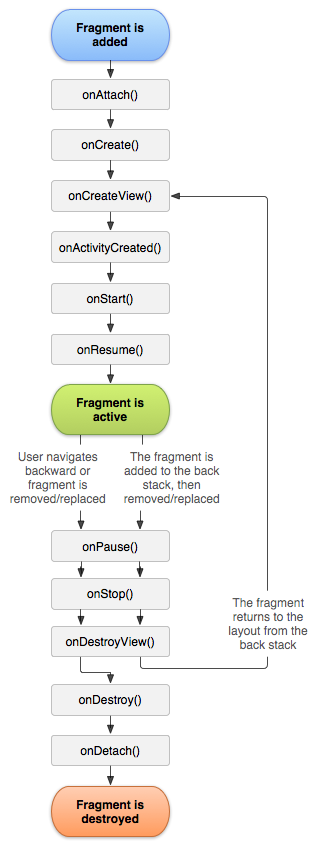
\includegraphics[width=0.5\textwidth]{images/fragments/lifecycle.png}
	\label{fig:fragcycle}
	\caption{The lifecycle of a fragment (while its activity is running).}
\end{figure}
Managing the lifecycle of a fragment is a lot like managing the lifecycle of an activity. Like an activity, a fragment can exist in three states:
\begin{description}
	\item[Resumed] The fragment is visible in the running activity.
	\item[Paused] Another activity is in the foreground and has focus, but the activity in which this fragment lives is still visible (the foreground activity is partially transparent or doesn't cover the entire screen).
	\item[Stopped] The fragment isn't visible. Either the host activity has been stopped or the fragment has been removed from the activity but added to the back stack. A stopped fragment is still alive (all state and member information is retained by the system). However, it is no longer visible to the user and is killed if the activity is killed.
\end{description}


\subsection{Creating a Fragment}
In Kotlin you delcare a Fragment by extending the Fragment class. 
\lstinputlisting[firstline=18,lastline=42	,language=Kotlin, caption={Creating a Fragment}, label=code:fragment]{srccode/fragments//RagecomicDetailFragment.kt}

This is what this code does:
\begin{enumerate}
	\item Declares RageComicDetailsFragment as a subclass of Fragment.
	\item An onCreate method which initialises the dependencies and or restores the state
\end{enumerate}

In most cases you need the following methods in order for a Fragment to work.

\begin{itemize}
	\item onCreate()
	The system calls this when creating the fragment. Within your implementation, you should initialize essential components of the fragment that you want to retain when the fragment is paused or stopped, then resumed.
	\item onCreateView()
	The system calls this when it's time for the fragment to draw its user interface for the first time. To draw a UI for your fragment, you must return a View from this method that is the root of your fragment's layout. You can return null if the fragment does not provide a UI.
	\item onPause()
	The system calls this method as the first indication that the user is leaving the fragment (though it doesn't always mean the fragment is being destroyed). This is usually where you should commit any changes that should be persisted beyond the current user session (because the user might not come back).
\end{itemize}
Also like an activity, you can preserve the UI state of a fragment across configuration changes and process death using a combination of onSaveInstanceState(Bundle), ViewModel, and persistent local storage. 

The most significant difference in lifecycle between an activity and a fragment is how one is stored in its respective back stack. An activity is placed into a back stack of activities that's managed by the system when it's stopped, by default (so that the user can navigate back to it with the Back button, as discussed in Tasks and Back Stack). However, a fragment is placed into a back stack managed by the host activity only when you explicitly request that the instance be saved by calling addToBackStack() during a transaction that removes the fragment.

\subsection{Adding a Fragment to an Activity}

Adding the fragment to an activity can either be done by declaring it in the XML layout file of the activity, or dynamically in the code by using FragmentTransactions.

\subsubsection{Adding a Fragment Dynamically}
First, you grab the FragmentManager by referencing supportFragmentManager.

Then, you ask that FragmentManager to start a new transaction by calling beginTransaction(). Next, you specify the add operation that you want by calling add and passing in:

\begin{enumerate}
\item The view ID of a container for the fragment’s view hierarchy in the activity’s layout. If you take a look at the layout you'll find single pane.
\item The fragment instance to be added.
\item A string that acts as a tag/identifier for the fragment instance. This allows the FragmentManager to later retrieve the fragment for you.
\end{enumerate}

You can also remove or replace fragments one by another. 

Finally, you ask the FragmentManager to execute the transaction by calling commit().

\lstinputlisting[firstline=137,lastline=140,language=Kotlin, caption={Replacing the fragment by using transactions.}, label=code:fragmentCode]{srccode/fragments/RagecomicListActivity.kt}

Of course your layout file should have a place holder for your Fragment.

\lstinputlisting[firstline=33,lastline=37,language=XML, caption={The XML layout file for an activity with a dynamic Fragment. The Framelayout servers as a place holder}, label=code:dynamicFragment]{srccode/fragments/layout-w900dp/ragecomic_list.xml}

As seen above, managing fragments in your activity requires the FragmentManager. 

Some things that you can do with FragmentManager include:

\begin{enumerate}
	\item Get fragments that exist in the activity, with findFragmentById() (for fragments that provide a UI in the activity layout) or \item findFragmentByTag() (for fragments that do or don't provide a UI).
	\item Pop fragments off the back stack, with popBackStack() (simulating a Back command by the user).
	\item Register a listener for changes to the back stack, with addOnBackStackChangedListener().
\end{enumerate}

\subsection{Communicating with the Activity}
You can  define a callback interface inside the fragment and require that the host activity implement it. When the activity receives a callback through the interface, it can share the information with other fragments in the layout as necessary.






\chapterimage{images/intents/intentchapterimage.jpg}

\chapter{Intents and Broadcastreceivers}


\begin{example}
	In this example we see an application which is able to convert speech into text.
	You can find the application here \cite{Buysse18}.
	This activity contains a button, which will create an special intent launching an Activity which is able to listen to speech, convert it to text and return its results.
	You will need an actual Android Device to test this. 
	
	The application is also  able to provide the user with a list of extra actions which he is able to perform. The choices are the following:
	\begin{itemize}
		\item Open a web-site with a given url (validate the URL)
		\item Open the contacts
		\item Open another Activity
		\item Open the dialer
		\item Search google
	\end{itemize}
	
\end{example}


\section{Intent}
Intents are objects which you can use for the following actions:


\begin{itemize}
	\item Explicitly start a particular Service or Activity using its class name (already seen in previous lessons)
	\item Implicitly start a particular Service or Activity
	\item Start an Activity or Service to perform an action with (or on) a particular piece of data
	\item Broadcast that an event has occurred
\end{itemize}

The two most important pieces of an Intent are the action and what Android refers to as the data.
If you were to create an Intent combining ACTION\_VIEW with a content Uri of https://google.com, and pass that Intent to Android via startActivity(), Android would know to find and open an activity capable of viewing that resource.


There are other criteria you can place inside an Intent
\begin{description}
	\item[Categories] A string containing additional information about the kind of component that should handle the intent.
	Any number of category descriptions can be placed in an intent, but most intents do not require a category.
	Your “main” activity will be in the LAUNCHER category, indicating it should show up on the launcher menu.
	\item[A MIME type]  indicating the type of resource you want to operate on.
	\item[Extras] which is a Bundle of other information you want to pass along to the receiver with the Intent, that the recipient might want to take advantage
\end{description}

If you specify the target component in your Intent , Android has no doubt where the Intent is supposed to be routed to and it will launch the named activity or application component.
This might be OK if the target recipient (e.g., the activity to be started) is in your application.

\begin{framed}
		This way of starting components (explicit) is definitely not recommended for invoking functionality in other applications.
		Component name are considered private to the application and are subject to change.
\end{framed}

There are two types of intents: explicit and implicit.

\subsection{Explicit Intent}
\textbf{An explicit intent} is one that you use to launch a specific app component, such as a particular activity or service in your app.
To create an explicit intent, define the component name for the Intent object, all other Intent properties are optional.

For example, if you want to start another activity from your application you could use the following code. 

\lstinputlisting[firstline=89,lastline=92,language=Kotlin, caption={Starting an explicit intent}, label=code:explicitIntent]{srccode/intents/fragments/MainActivityFragment.kt}

The Intent is built inside the MainActivity and not outside. You cannot make it wrong and accidentally forget an extra. 

\lstinputlisting[firstline=23,lastline=32,language=Kotlin, caption={Generating the intent in the Activity.}, label=code:explicitIntent]{srccode/intents/activities/MainActivity.kt}

\subsection{Implicit intent}
An implicit intent specifies an action that can invoke any app on the device able to perform the action.
Using an implicit intent is useful when your app cannot perform the action, but other apps probably can and you'd like the user to pick which app to use.

For example, if you need a contact from the Contact on your user's phone you could generate an Intent and start an activity to get it. 

\lstinputlisting[firstline=58,lastline=61,language=Kotlin, caption={Starting an implicit intent to find a contact from the contact app }, label=code:explicitIntent]{srccode/intents/fragments/MainActivityFragment.kt}


\begin{framed}
It's good practice to determine if your call will resolve to an Activity before calling startActivity. In our example application we have created the method checkForCompatibility.
\end{framed}

\lstinputlisting[firstline=121,lastline=144,language=Kotlin, caption={Check if there is an Activity which is able to handle the intent}, label=code:explicitIntent]{srccode/intents/fragments/MainActivityFragment.kt}

\subsection{Allow to start your Activity from another app}

\begin{figure}
	\includegraphics[width=\textwidth]{images/intents/intentresolution.png}
	\caption{Android OS uses filters to pinpoint the set of Activities, Services, and Broadcast receivers that can handle the Intent with help of specified set of action, categories, data scheme associated with an Intent.
		You will use <intent-filter> element in the manifest file to list down actions, categories and data types associated with any activity, service, or broadcast receiver.}
	\label{fig:intentresolution}
\end{figure}

To allow other apps to start your activity, you need to add an intent-filter element in your manifest file for the corresponding activity element.
In order to properly define which intents your activity can handle, each intent filter you add should be as specific as possible in terms of the type of action and data the activity accepts.
The system may send a given Intent to an activity if that activity has an intent filter that fulfils the following criteria of the Intent object:

\begin{itemize}
	\item Action : A string naming the action to perform.
	\item Data : A description of the data associated with the intent.
	\item Category: Provides an additional way to characterize the activity handling the intent, usually related to the user gesture or location from which it's started.
\end{itemize}

For example, here's an activity declaration with an intent filter to receive an ACTION\_SEND intent when the data type is text:

\lstinputlisting[firstline=48,lastline=54,language=kxml, caption={An example intent filter}, label=code:explicitIntent]{srccode/intents/explicit.kt}

\section{Broadcastreceiver}
So far, you’ve looked at using Intents to start new application components, but you can also use Intents to broadcast messages anonymously between components via the sendBroadcast() method.
As a system-level message-passing mechanism, Intents are capable of sending structured messages across process boundaries.
As a result, you can implement BroadcastReceivers to listen for, and respond to, these Broadcast Intents within your applications.

Within your application, construct the Intent you want to broadcast and call sendBroadcast() to send it.
Set the action, data, and category of your Intent in a way that lets BroadcastReceivers accurately determine their interest.

\subsection{Receiving a broadcast (without the manifest)}
To receive such a broadcast in an activity (or a fragment), you will need to do four things.

\begin{enumerate}
	\item You will need to create an instance of your own subclass of BroadcastReceiver.
	The only method you need to (or should) implement is onReceive(), which will be passed the Intent that was broadcast, along with a Context object that, in this case, you will typically ignore. 
	\item Second, you will need to create an instance of an IntentFilter object, describing	the sorts of broadcasts you want to receive. 
	Most of these filters are set up to watch for a single broadcast Intent action.
	\item You will need to call registerReceiver(), typically from onStart() or onResume() of your activity or fragment, supplying your BroadcastReceiver and your IntentFilter.
	\item You will need to call unregisterReceiver(), typically from onStop() or onPause() of your activity or fragment, supplying the same BroadcastReceiver instance you provided	to registerReceiver().
\end{enumerate}

\subsection{Receiving a broadcast (with the manifest)}
You can also tell Android about broadcasts you wish to receive by adding a <receiver> element to your manifest, identifying the class that implements your BroadcastReceiver (via the android:name attribute), plus an <intent-filter> that describes the broadcast(s) you wish to receive:

\lstinputlisting[firstline=57,lastline=61,language=kxml, caption={Receiving a Broadcast with the manifest}, label=code:explicitIntent]{srccode/intents/explicit.kt}

The good news is that this BroadcastReceiver will be available for broadcasts occurring at any time.
There is no assumption that you have an activity already running that called registerReceiver().
The bad news is that the instance of the BroadcastReceiver used by Android to process a broadcast will live for only so long as it takes to execute the onReceive() method.
At that point, the BroadcastReceiver is discarded.
Hence, it is not safe for a manifest-registered BroadcastReceiver to do anything that needs to run after onReceive() itself completes, such as forking a thread.
After all, Android may well terminate the process within milliseconds, if there is no other running component in the process.
Moreover, onReceive() is called on the main application thread and may freeze your UI.
\chapterimage{images/recycler/recycling.jpg}
\chapter{Recyclerview}
In 2014, Google released RecyclerView, via the Android Support package.
Developers can add the recyclerview-v7 to their projects and use RecyclerView.
In this chapter, we will review RecyclerView from the ground up, starting with basic
operation.

Before you are able to use the recylceview,  open build.gradle (app) and add the dependencies needed.


\begin{lstlisting}
dependencies {
	implementation 'com.android.support:recyclerview-v7:28.0.0'
}
\end{lstlisting}


\begin{example}
	The code examples for this chapter is the same code example as for the Fragment application, where we will focus on the  \lstinline!RecyclerView!.
\end{example}

\section{What is a recyclerview}
The \lstinline!RecyclerView! is a new \lstinline!ViewGroup! that is prepared to render any adapter-based view.
It is supposed to be the successor of \lstinline!ListView! and \lstinline!GridView!, and it can be found in the \lstinline!support-v7! version.
One of the reasons is that \lstinline!RecyclerView! has a more extensible framework, especially since it provides the ability to implement both horizontal and vertical layouts.
Use the RecyclerView widget when you have data collections whose elements change at runtime based on user action or network events.

To use a \lstinline!RecyclerView!, you will need the following things:
\begin{enumerate}
	\item \lstinline!RecyclerView.Adapter! - To handle the data collection and bind it to the view
	\item A layout file defining the row layout in the \lstinline!RecyclerView!.
Just a note here: when you create the item layout of the \lstinline!RecyclerView! don’t forget to add the following lines in the ViewGroup container of the layout.
This lines of code will add the ripple effect to the RecyclerView elements.
	\begin{enumerate}
		\item  \lstinline!android:clickable="true"!
		\item \lstinline!android:focusable="true"!
		\item \lstinline!android:foreground="?android:attr/selectableItemBackground"!
	\end{enumerate}
	\item \lstinline!LayoutManager! - Helps positioning the items
	\item \lstinline!ItemAnimator! - Helps with animating the items for common operations such as Addition or Removal of item
\end{enumerate}


\section{Basic operation}
When the list is first populated, it creates and binds some view holders on either side of the list.
For example, if the view is displaying list positions 0 through 9, the \lstinline!RecyclerView! creates and binds those view holders, and might also create and bind the view holder for position 10.
That way, if the user scrolls the list, the next element is ready to display.

As the user scrolls the list, the \lstinline!RecyclerView! creates new view holders as necessary.
It also saves the view holders which have scrolled off-screen, so they can be reused.
If the user switches the direction they were scrolling, the view holders which were scrolled off the screen can be brought right back.
On the other hand, if the user keeps scrolling in the same direction, the view holders which have been off-screen the longest can be re-bound to new data.
The view holder does not need to be created or have its view inflated; instead, the app just updates the view's contents to match the new item it was bound to.

When the displayed items change, you can notify the adapter by calling an appropriate \lstinline!RecyclerView.Adapter.notify()! method.
The adapter's built-in code then rebinds just the affected items.

\section{Components and Workflow}

\begin{figure}
	\includegraphics[width=\textwidth]{images/recycler/components.png}
	\caption{ \lstinline!RecyclerView! is a major enhancement over \lstinline!ListView!.
It contains many new features like \lstinline!ViewHolder!, \lstinline!ItemDecorator!, \lstinline!LayoutManager!, and \lstinline!SmoothScroller!.
But one thing that certainly gives it an edge over the \lstinline!ListView! is; the ability to have animations while adding or removing an item.}
	\label{fig:recyclercomponents}
\end{figure}


\subsection{RecyclerView.Adapter}
\lstinline!RecyclerView! uses an adapter to help convert our model data into visual representations.
A \lstinline!RecyclerView.Adapter!  uses a generic to identify a \lstinline!ViewHolder! that will be responsible for doing the work to actually tie model data to row widgets.

RecyclerView.Adapter has three abstract methods that need to be implemented.

\begin{enumerate}
	\item \lstinline!getItemCount()!, which fills the same role as does \lstinline!getCount()! indicating how many items there will be in the RecyclerView
	\item \lstinline!onCreateViewHolder()!  needs to create, configure,	a ViewHolder for a particular row of our list.
	It is passed two parameters:
	\begin{enumerate}
		\item a \lstinline!ViewGroup! that will hold the views managed by the holder, mostly for use
		with layout inflation, and
		\item an \lstinline!Int! that is the particular view type we are using, for cases where we have
		multiple view types
	\end{enumerate}
	\item \lstinline!onBindViewHolder()!
	is responsible for updating a ViewHolder based upon the
	model data for a certain position .
\end{enumerate}


\lstinputlisting[firstline=43,lastline=64,language=kotlin, caption={The definitions of the methods for a RecyclerView.adapter}, label=code:rec1]{srccode/recyclerview/recycle.kt}

\subsection{ViewHolder}
The \lstinline!RecyclerView.ViewHolder! is responsible for binding data as needed from our model into the widgets for a row in our list.
However, other than needing to use the base class of \lstinline!RecyclerView.ViewHolder!, there is no other particular protocol that is mandated between the adapter and the view holder.
You can invent your own API.

\lstinputlisting[firstline=71,lastline=77,language=kotlin, caption={The ViewHolder definition.}, label=code:rec1]{srccode/recyclerview/recycle.kt}


\subsection{LayoutManagers}
After adding a \lstinline!RecyclerView! to the \lstinline!Activity!, the first thing we do is call \lstinline!setLayoutManager()!,
which will associate a \lstinline!RecyclerView.LayoutManager! with our \lstinline!RecyclerView!, for example a \lstinline!LinearLayoutManager!.
\lstinline!RecyclerView! knows absolutely nothing about how to lay out its children.
That work is delegated to a \lstinline!RecyclerView.LayoutManager!, so that different approaches can be plugged in as needed.

There are three concrete subclasses of the abstract \lstinline!RecyclerView.LayoutManager! base class that ship with \lstinline!recyclerview-v7! :
\begin{enumerate}
	\item \lstinline!LinearLayoutManager! , which implements a vertically-scrolling list
	\item \lstinline!GridLayoutManager! ,
	which implements a two-dimensional vertically-
	scrolling list
	\item \lstinline!StaggeredGridLayoutManager! , which implements a staggered grid, which has columns of cells like a \lstinline!GridView!, but where the cells do not have to all have the same size.
\end{enumerate}

In our example we have defined the LayoutManager in the XML.
This is not a best practise and will be changed in the next iteration of this course.

\subsection{ItemAnimator}
\lstinline!RecyclerView.ItemAnimator! is a class that defines the animations performed on items and will animate \lstinline!ViewGroup! changes such as add/delete/select notified to the adapter.
DefaultItemAnimator is a basic animation available by default with the RecyclerView.

To customize the DefaultItemAnimator add an item animator to the RecyclerView.

\section{Responding to Clicks}
Even though displaying elements in \lstinline|RecyclerView| is better, in terms of performance, than its predecessors,  \lstinline|ListView |and  \lstinline|GridView|, it is not simple to add a clicklistener.

In previous version of Android, mainly where we used Java, we had to create interfaces -, implement them and assign them to the adapter.
With the knowledge of function parameters and lambda expressions in Kotlin hower, we can start adding a click handler to our RecyclerView in a more elegant way.

Android has defined an Interface, which is part of the \lstinline|View|  class: \lstinline|View.OnClickListener|.
It only contains one methode, namely \lstinline|onClick(View v)| which is called whenever a view has been clicked.

\subsection*{Extend the Adapter}
We  need a new  parameter in the definition of our Adapter: the click listener function which we will define as a  function parameter.
The clickListener parameter is a val, meaning that it’s constant in our Adapter.
It does not need a new function paramter, as every view has a tag (\lstinline|View.tag|) that can be used to store data related to that view.

The documentation states: \textit{Tags are essentially an extra piece of information that can be associated with a view.
They are most often used as a convenience to store data related to views in the views themselves rather than by putting them in a separate structure.}

In our case, each item in the \lstinline|RecyclerView| keeps a reference to the comic it represents which  allows us to reuse a single listener for all comics in the list.

\lstinputlisting[firstline=5,lastline=13,language=kotlin, caption={Extending the Adapter}, label=code:rec1]{srccode/recyclerview/recycle.kt}	

\subsection*{Implementing the ViewHolder \& ClickListener}
We want the individual items in the list to handle click events.
These items are managed by the \lstinline|ViewHolder|.
In our example, we called the view holder: \lstinline|ViewHolder|.
Whenever the \lstinline|RecyclerView| assigns (new) content to the item, our Adapter calls \lstinline|bind()| of the specific \lstinline|ViewHolder| responsible for the item view.

Therefore, \lstinline|bind()| is the logical place to also ensure the item sends back the correct item data whenever it is clicked.
We add a second parameter to the  \lstinline|bind()| function: a function parameter for the click listener.

\lstinputlisting[firstline=52,lastline=64,language=kotlin, caption={Binding the ViewHolder}, label=code:rec1]{srccode/recyclerview/recycle.kt}

\subsection*{Handle the click events}
The Adapter and the \lstinline|ViewHolder| are ready to process click events.
The last step is to handle clicks.
We need to implement this functionality in the  \lstinline|init| part of the class because the primary constructor cannot contain any code.
Initialization code can be placed in initializer blocks, which are prefixed with the \lstinline|init| keyword.

What you can see in the code is that the onClickListener is implemented using a functional type.

\lstinputlisting[firstline=16,lastline=41,language=kotlin, caption={The ViewHolder definition.}, label=code:rec1]{srccode/recyclerview/recycle.kt}

\section{CardView}
\lstinline!Cards! are a popular visual metaphor in mobile development.
Dividing content collections (or aspects of a larger piece of content) into cards makes it clearer how you can reorganize that content to fit various screen sizes and orientations.
In some cases, you might have a single column of cards, while in other cases, you have cards
arranged more laterally.

In 2014, Google released cardview-v7, another library in the Android Support package, that offers a CardView.
CardView is a simple subclass of FrameLayout, designed to provide a card UI, consisting of a rounded rectangle and a drop shadow.
In particular, CardView will use Android 5.0’s default drop shadows based on widget elevation, while offering emulated drop shadows on earlier Android releases.
This
way, you can get a reasonably consistent look going back to API Level 7.
To use this, you will have to add the cardview-v7 library to your app project.
Android Studio users can just add a dependency on the cardview-v7 artifact in the Android Support repository

\section{Example}

\begin{example}
In the repository found here \cite{Buysse2017}, we find an example demonstrating the principles explained above.
Moreover, it makes use of a Fragment with a Recyclerview.
It uses Butterknife as already demonstrated in previous example.
For loading the images it makes use of the Picasso library (see \cite{Square2017}).
This example is from previous year, where Java was still used.
\end{example}




\chapterimage{images/mvvm/header.png}


\chapter{Architecture: from MVC to MVVM}

\section{Why}
A software project using a well-thought out architecture saves time: it allows for development of new features, it helps the programmer when existing features need to be changed, it is easy to test and provides the programmer with a sense of confidence, and so on. 
There are many different ways to architect an (Android) application: MVC, MVVM, MVI, MVP,\ldots 
Each have there own pros and cons, and it's up to the developer to know when the pick which.

The core idea of each architecture is the same however: separation of concerns.
The responsibilities of each class or module should be clearly defined and all these component should work together in a well-structured way. 
How this is done is different for each architecture. 

Some architectures are better supported by the (Android) framework than others. 
``Base'' Android is mostly MVC (Model, View, Controller), but with the release of the Android Architecture Components came more support for a MVVM (Model, View, ViewModel) approach.
The next two sections cover both, but in this course we will study MVVM more in depth. 


%Base Android: Controller is Activity/Fragment, Model is the Model, View is Layout
%Probleem is dat Controller in Android zo gelinkt is aan architectuur dat die niet getest kan worden.
%Moet ook veel doen: model bijhouden, updaten, UI listenen,...
%Later zal VM de repo bijhouden, activity wordt steeds kleiner

\section{MVC}
MVC is one of the more common architectural software patterns.
It divides your code into three interconnected parts \cite{mvc-mvp-mvv-on-android}:

\begin{description}
	\item[Model:] the central data and state of the application, together with the business logic.
	\item[View:] the representation of the model. Its responsibility is to render the UI.
	\item[Controller:] acts as an agent between the model and the view. 
		When the view receives user input, the controller will interact with the model to attain the desired effects.
\end{description}

Figure \ref{fig:MVCdiagram} illustrates the role of standard Android Components such as layout files, \lstinline!Activities! and \lstinline!Fragments! in MVC.
Normally MVC is a good way to architect your application, but in Android specifically there are some issues:

\begin{enumerate}
	\item Unit Testing the \lstinline!Activities! and \lstinline!Fragments! is extremely difficult because they are so tied in to the Android Framework.
	``God'' objects such as Context and the \lstinline!Activity! life cycle all stand in the way of easy testing.
	\item \lstinline!Activities! and \lstinline!Fragments! as controllers have many responsibilities. 
	They have to keep the UI (View) up-to-date, interact with databases or remote API's, correctly implement the life cycle,\ldots
	This makes for lots of code which becomes harder to maintain over time.
	\item Controllers and Views are tightly coupled: changing something in a layout file is very likely to mean changes in the controller as well. 
\end{enumerate}

\begin{figure}[ht]
	\centering
	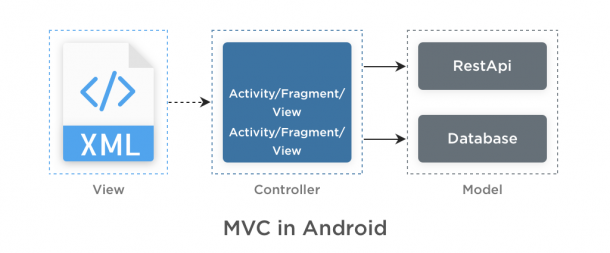
\includegraphics[width=\textwidth]{images/mvvm/MVC_diagram.png}
	\label{fig:MVCdiagram}
	\caption{A diagram illustrating the MVC architecture in Android. From \cite{simform}.}
\end{figure}

Luckily, there is a better way to organize your code: through architectural patterns such as MVVM, MVI, MVP \ldots

All have gained some popularity in the Android community, but the recently released architecture components \cite{architectureComponents} focus quite heavily on MVVM.
In this course we will make much use of these components and as such use MVVM as our architecture of choice.

\section{MVVM}
In this section we explore the MVVM architecture step-by-step. 
We start by looking at the concept of a \lstinline!ViewModel! class, and how it helps us with the issue of configuration changes.
After that has been made clear, we use this \lstinline!ViewModel! class to be part of an MVVM architecture. 
Lastly we look at another use case for the \lstinline!ViewModel! class: a way to allow our UI to update automatically once the model changes. 
This will be done using by binding the data from the \lstinline!ViewModel! to the layoutfile.

\subsection{ViewModel as a way to survive configuration changes}
We have discussed the problem of saving and restoring state already in section \ref{sec:saveAndRestoreState}. 
There the \lstinline!onSaveInstanceState! and \lstinline!onCreate! methods were proposed as a solution.
A short example of this can be seen in listing \ref{code:basicMVC}.

\lstinputlisting[language=Kotlin, 
caption={A simple application with a \lstinline!TextView!, an \lstinline!EditText! and a \lstinline!Button!.
	After pressing the button, the text in the \lstinline!TextView! is updated with the user's input in the \lstinline!EditText!.
	Saving and Restoring UI state is done using the \lstinline!onSaveInstanceState! method.},
label=code:basicMVC]{srccode/mvvm/MVC_simple/app/src/main/java/be/hogent/nativeapps/mvc_example/MainActivity.kt}

However, there is another solution: using a \lstinline!ViewModel! class.
This class is part of the Android Lifecycle Architecture Components \cite{viewModelOfficial}.
While the concept of a viewmodel isn't specific to Android, this implementation is of particular interest to us because it ties in to the \lstinline!Activity! lifecycle.

The \lstinline!ViewModel! class is part of the Android Lifecycle Extensions Library.
To use this library it has to be added as a dependency of your application.
This means the following line has to be added to your app module's gradle file:

\begin{android}
	implementation "android.arch.lifecycle:extensions:1.1.1"
\end{android}


A generic viewmodel class is used as part of an MVVM architecture (more on that later), and its job is to hold all elements of the model that are exposed in the UI.

This reduces the size and complexity of what would normally be the controller.
In our case, it is exactly those pieces of data that we normally lose during configuration changes.
We could make that generic viewmodel class \lstinline!Serializable! and use \lstinline!onSaveInstanceState! and \lstinline!onCreate! to save and restore it, but there is an easier way. 

The ViewModel class that is a part of the Android Architecture Components isn't one that you create yourself using a regular constructor, but by using a \lstinline!ViewModelProvider! \cite{viewModelProvider}.
In the \lstinline!onCreate! function of your \lstinline!Fragment! or \lstinline!Activity! you use the following line of code to instantiate your \lstinline!ViewModel!.


\begin{android}
val model = ViewModelProviders.of(this).get(MyViewModel::class.java)	
\end{android}

The \lstinline!this! refers to the \lstinline!Activity! itself, and links the \lstinline!ViewModel! to the \lstinline!Activity's! lifecycle.

\lstinline!ViewModelProviders! keeps a list of all active life cycles and the associated \lstinline!ViewModels!.
\footnote{This becomes especially important when using \lstinline!ViewModels! for sharing data between \lstinline!Fragments!.
Using the example of a dual-pane layout: both the \lstinline!ListFragment! and \lstinline!DetailFragment! would need to specify the \lstinline!Activity! that hosts them both when creating the \lstinline!ViewModel! in order to both receive the same instance. 
More information on this can be found in \cite{shareDataBetweenFragments}.}

When a configuration change occurs, the \lstinline!ViewModelProvider! still has a reference to the created \lstinline!ViewModel! and can just return it.
This alleviates the need for \lstinline!onSaveInstanceState! for configuration change state changes. 

An example implementation can be seen in \ref{code:viewModelActivity} (the \lstinline!Activity! class) and \ref{code:viewModelSimple} (the \lstinline!ViewModel! class).
In more realistic applications the \lstinline!ViewModel! would hold much more than just one piece of UI information.

Every part of the UI that gets data from the model should be retained in the \lstinline!ViewModel!.

\lstinputlisting[language=Kotlin,
caption={A very simple application with a \lstinline!TextView!, an \lstinline!EditText! and a \lstinline!Button!.
	After pressing the button, the text in the \lstinline!TextView! is updated with the user's input in the \lstinline!EditText!.
	Saving and Restoring UI state is done using a \lstinline!ViewModel!.},
label=code:viewModelActivity]{srccode/mvvm/ViewModel_simple/app/src/main/java/be/hogent/nativeapps/mvc_example/MainActivity.kt}

\lstinputlisting[language=Kotlin,
caption={The InputViewModel class that is used in listing \ref{code:viewModelActivity}.
	It extends the abstract ViewModel class from the Android Architecture Components.},
label=code:viewModelSimple]{srccode/mvvm/ViewModel_simple/app/src/main/java/be/hogent/nativeapps/mvc_example/InputViewModel.kt}

\subsection{ViewModel with Data Binding and LiveData as part of an MVVM architecture}

Extracting the UI state from the \lstinline!Activity! as done in the previous section is the first step towards a full MVVM architecture.
MVVM is composed of 3 parts, as illustrated in \ref{fig:MVVMdiagram}
\begin{description}
	\item[Model:] the central data and state of the application, together with the business logic.
	\item[View:] the representation of the model. Its responsibility is to render the UI.
				In contrast with MVC, in MVVM the  \lstinline!Activity! or  \lstinline!Fragment! is also considered part of the View.
	\item[ViewModel:] a container that wraps (part of) the model and provides observable data needed by the view.
	It also provides hooks for the view to pass events to the model. The ViewModel is not tied to the view however.
\end{description}

\begin{figure}[ht]
	\centering
	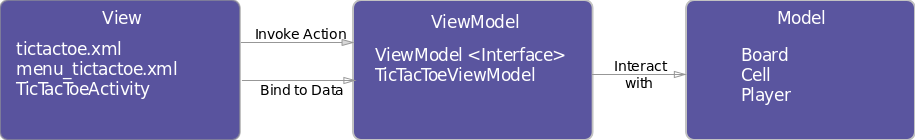
\includegraphics[width=\textwidth]{images/mvvm/MVVM.png}
	\label{fig:MVVMdiagram}
	\caption{A diagram illustrating the MVVM architecture in Android.
		Here it is applied to a Tic-Tac-Toe game.
		From \cite{mvc-mvp-mvv-on-android}.}
\end{figure}

The responsibilities and direction of communication are a bit different from what we are used to.
The \lstinline!Activity! or \lstinline!Fragment! will no longer configure each piece of the UI, instead the UI gets its data from a \lstinline!ViewModel! directly.
Actions aren't registered in the \lstinline!Activity!, but are sent from layout to the \lstinline!ViewModel!, which in turn communicates with the model.
Communication with the Android Framework in order to switch screens will have to be done in a way that requires complete separation between the ViewModel and the \lstinline!Activity! or \lstinline!Fragment!.
Each of these three requirements are discussed in a separate section.

\subsubsection{Binding the ViewModel to the View}
If we want the View to bind to data from the \lstinline!ViewModel! 
This is done using the Data Binding library \cite{dataBinding}.
It allows you to add a link to a \lstinline!ViewModel! (or other model classes) directly into your layout files.

Any UI component that needs a piece of data from the \lstinline!ViewMode!l can request it directly from the \lstinline!ViewModel!.
This reduces the role of the \lstinline!Activity! even more: it is no longer responsible for updating the \lstinline!View!.

The first step is transforming the normal layout into one that supports data binding.
This involves creating a variable in the layout file that will hold a reference to the ViewModel.
Listing \ref{code:dataBindingXMLvariable} illustrates this step.

\lstinputlisting[language=XML, firstline=2,lastline=8,
caption={The entire layout is wrapped by a <layout> tag, and a variable is defined to hold the ViewModel},
label=code:dataBindingXMLvariable]{srccode/mvvm/ViewModel_DataBinding_LiveData/app/src/main/res/layout/activity_main.xml}

UI components can then reference this variable when they require a piece of UI state, as shown in listing \ref{code:dataBindingXMLreference}.

\lstinputlisting[language=XML, firstline=16,lastline=21,
caption={XML attributes can reference the variable to fill their values.},
label=code:dataBindingXMLreference]{srccode/mvvm/ViewModel_DataBinding_LiveData/app/src/main/res/layout/activity_main.xml}

\subsubsection{Automatically updating the UI on state changes}
The matter of updating the state of the UI when a user interacts with it can be solved using the LiveData Architecture Component \cite{liveData}.

A LiveData object is an observable object. This means that other objects can first register and subsequently listen to changes in the value of that object.
This functionality alone could also be provided using Observable objects \cite{observable}.
LiveData however has much more to offer: it is completely linked with the listener's lifecycle. This means no problems during configuration changes, no memory leaks, no updates send to inactive (and possibly destroyed) listeners resulting in crashes\ldots

Using LiveData means making minor changes to both the \lstinline!ViewModel! and the \lstinline!Activity!, as seen in listing \ref{code:dataBindingViewModel}

In the \lstinline!ViewModel! the attributes are now wrapped inside \lstinline!LiveData! objects.
This provides all lifecycle and observable functionality. 

\lstinputlisting[language=Kotlin,
caption={Attributes in the \lstinline!ViewModel! are wrapped inside \lstinline!LiveData! objects. Sometimes some extra initialization code is needed.},
label=code:dataBindingViewModel]{srccode/mvvm/ViewModel_DataBinding_LiveData/app/src/main/java/be/hogent/nativeapps/mvc_example/InputViewModel.kt}

In the \lstinline!Activity! there are 3 things to do:
\begin{inparaenum}[(i)]
	\item ask for the binding with the layout file,
	\item binding the \lstinline!ViewModel! to the layout and
	\item setting the \lstinline!LifeCycleOwner!.
\end{inparaenum}

We need the binding to set up the link with the variables defined in the layout file. 
Setting the \lstinline!LifeCycleOwner! is needed when using \lstinline!LiveData!. 
Without this step the LiveData objects can't know when their listeners are active or not. All three steps are illustrated in listing \ref{code:dataBindingActivity}.


\lstinputlisting[language=Kotlin,firstline=14, lastline=31,
caption={Attributes in the \lstinline!ViewModel! are wrapped inside \lstinline!LiveData! objects. Sometimes some extra initialization code is needed.},
label=code:dataBindingActivity]{srccode/mvvm/ViewModel_DataBinding_LiveData/app/src/main/java/be/hogent/nativeapps/mvc_example/MainActivity.kt}

\subsubsection{Responding to events that require Activity or Fragment}
A very important aspect of the \lstinline!ViewModel! is that it should \textbf{never} hold any references to a \lstinline!View!, be it a \lstinline!Activity! or a \lstinline!Fragment!.
This is because \lstinline!ViewModels! are designed to survive configuration changes, and \lstinline!Views! are not.
So holding a reference to a \lstinline!View! that has been destroyed will lead to crashes. 

This leads to the problem of how to respond to user interactions that require, for example, a new screen to be shown.
To start a new \lstinline!Activity! or \lstinline!Fragment! you need to have a reference to one.
But we can't, because a \lstinline!ViewModel! can't hold these references!

To solve this, we allow \lstinline!Activities! and \lstinline!Fragments! to observe special events produced by their \lstinline!ViewModels!.
Using the same \lstinline!LiveData! library from before we can make a special kind of observable object 
(an instance of \lstinline!SingeLiveEvent!\footnote{\url{https://raw.githubusercontent.com/hdeweirdt/CriminalIntent/viewmodel/app/src/main/java/com/deweirdt/harm/criminalIntent/util/SingleLiveEvent.kt}}) 
that we will cause to update whenever the user indicates they want to go to another screen.
The \lstinline!Activity! or \lstinline!Fragment! will observe this object and react to the event by following the usual steps to start a new \lstinline!Activity! or \lstinline!Fragment!.

The \lstinline!ViewModel! code is illustrated in figure \ref{code:ViewModelEvent}.
The \lstinline!Fragment! code is illustrated in figure \ref{code:FragmentEvent}.
	
\begin{lstlisting}[language=Kotlin, label=code:ViewModelEvent,
caption={The \lstinline!ViewModel! has one \lstinline!SingeLiveEvent! for each interaction that eventually requires action from a \lstinline!Activity! or \lstinline!Fragment!.
The \lstinline!onButtonClicked! functions are referenced in the layout files.}]
val suspectButtonEvent = SingleLiveEvent<Unit>()

fun onSuspectButtonClicked(button: View) {
	suspectButtonEvent.call()
}
\end{lstlisting}

\begin{lstlisting}[language=Kotlin,label=code:FragmentEvent,
caption={The \lstinline!Activities! or \lstinline!Fragments! observe the events from the  \lstinline!ViewModel!, and respond by creating a new \lstinline!Activity! or \lstinline!Fragment!}]
 override fun onStart() {
	super.onStart()
	mCrimeViewModel.suspectButtonEvent.observe(this, Observer { suspectButtonClicked() })
}
private fun suspectButtonClicked() {
	val pickContact = Intent(Intent.ACTION_PICK, ContactsContract.Contacts.CONTENT_URI)
	startActivityForResult(pickContact, REQUEST_CONTACT)
}
\end{lstlisting}
\chapterimage{images/persistency/persistence.jpg}

\chapter{Persistence}
In this Chapter we will review some of the persistence methods use in Android. We will have a look into saving a small portion of data and a more structured (relational) type of data.

\section{Shared preferences}
If you have a relatively small collection of key-values that you'd like to save, you should use the SharedPreferences APIs. A SharedPreferences object points to a file containing key-value pairs and provides simple methods to read and write them. Each SharedPreferences file is managed by the framework and can be private or shared.

\subsection{Creating shared preferences}
Using the SharedPreferences class, you can create named maps of name/value pairs that can be persisted across sessions and shared among application components running within the same application sandbox. To create or modify a Shared Preference, call getSharedPreferences on the current Context, passing in the name of the Shared Preference to change.

Shared Preferences are stored within the application’s sandbox, so they can be shared between an application’s components but aren’t available to other applications. To modify a Shared Preference, use the SharedPreferences.Editor class. Get the Editor object by calling edit on the Shared Preferences object you want to change.

To save edits, call apply on the Editor object to save the changes asynchronously.
\begin{android}
SharedPreferences mySharedPreferences = getSharedPreferences(MY_PREFS, 
Activity.MODE_PRIVATE);
SharedPreferences.Editor editor = mySharedPreferences.edit();
// Store new primitive types in the shared preferences object.
editor.putBoolean("isTrue", true);
editor.putFloat("lastFloat", 1f);
editor.putInt("wholeNumber", 2);
editor.putLong("aNumber", 3l);
editor.putString("textEntryValue", "Not Empty");
editor.apply();
\end{android}


\subsection{Retrieving shared preferences}
Accessing Shared Preferences, like editing and saving them, is done using the getSharedPreferences method. Use the type-safe get methods to extract saved values. Each getter takes a key and a default value (used when no value has yet been saved for that key.)

\begin{android}
// Retrieve the saved values.
boolean isTrue = mySharedPreferences.getBoolean("isTrue", false);
float lastFloat = mySharedPreferences.getFloat("lastFloat", 0f);
int wholeNumber = mySharedPreferences.getInt("wholeNumber", 1);
long aNumber = mySharedPreferences.getLong("aNumber", 0);
String stringPreference =
mySharedPreferences.getString("textEntryValue", "");
\end{android}

\section{SQLLite}
Using SQLite you can create fully encapsulated relational databases for your applications. Use them to store and manage complex, structured application data. Android databases are stored in the \texttt{/data/data/<package\_name>/databases} folder on your device (or emulator). All databases are private, accessible only by the application that created them.

\subsection{Define your Schema}
One of the main principles of SQL databases is the schema: a formal declaration of how the database is organized. The schema is reflected in the SQL statements that you use to create your database. You may find it helpful to create a companion class, known as a contract class, which explicitly specifies the layout of your schema in a systematic and self-documenting way.

A contract class is a container for constants that define names for URIs, tables, and columns. The contract class allows you to use the same constants across all the other classes in the same package. This lets you change a column name in one place and have it propagate throughout your code.

A good way to organize a contract class is to put definitions that are global to your whole database in the root level of the class. Then create an inner class for each table that enumerates its columns.

Note: By implementing the BaseColumns interface, your inner class can inherit a primary key field called \_ID that some Android classes such as cursor adaptors will expect it to have. It's not required, but this can help your database work harmoniously with the Android framework.


\subsection{Introducing the SQLiteOpenHelper}
SQLiteOpenHelper is an abstract class used to implement the best practice pattern for creating, opening, and upgrading databases. By implementing an SQLite Open Helper, you hide the logic used to decide if a database needs to be created or upgraded before it’s opened, as well as ensure that each operation is completed efficiently. It’s good practice to defer creating and opening databases until they’re needed. The SQLiteOpen Helper caches database instances after they’ve been successfully opened, so you can make requests to open the database immediately prior to performing a query or transaction. For the same reason, there is no need to close the database manually unless you no longer need to use it again.

\begin{framed}
	Database operations, especially opening or creating databases, can be time consuming. To ensure this doesn’t impact the user experience, make all database transactions asynchronous. Make sure you use the same connection when writing and reading to the database (where locking is implemented).
\end{framed}

To access a database using the SQLite Open Helper, call getWritableDatabase or getReadableDatabase to open and obtain a writable or read-only instance of the underlying database, respectively.

You need to override the following methods to create and update your database.
\begin{enumerate}
	\item onCreate() - is called by the framework, if the database is accessed but not yet created.
	\item onUpgrade() - called, if the database version is increased in your application code. This method allows you to update an existing database schema or to drop the existing database and recreate it via the onCreate() method.
	\item  onOpen() - This method is called after the database connection has been configured and after the database schema has been created, upgraded or downgraded as necessary.
\end{enumerate}

\begin{framed}
It is good practice to create a separate class per table. This class defines static onCreate() and onUpgrade() methods. These methods are called in the corresponding methods of SQLiteOpenHelper. This way your implementation of SQLiteOpenHelper stays readable, even if you have several tables.
\end{framed}

\subsubsection{Some considerations}
You should keep the following Android-specific considerations in mind when designing your database.
\begin{enumerate}
	\item Files (such as bitmaps or audio fi les) are not usually stored within database tables. Use a string to store a path to the fi le, preferably a fully qualifi ed URI.
	\item Although not strictly required, it’s strongly recommended that all tables include an auto-increment key field as a unique index field for each row. If you plan to share your table using a Content Provider, a unique ID field is required.
\end{enumerate}

\subsection{Query a database}
Each database query is returned as a \texttt{Cursor}. This lets Android manage resources more efficiently by retrieving and releasing row and column values on demand. To execute a query on a Database object, use the query method with the necessary parameters.

\subsubsection{Cursor}
A query returns a Cursor object. A Cursor represents the result of a query and basically points to one row of the query result. This way Android can buffer the query results efficiently; as it does not have to load all data into memory.

To extract values from a Cursor, first use the \texttt{moveTo<location>} method to position the cursor at the correct row of the result Cursor, and then use the type-safe \texttt{get<type>} methods (passing in a column index) to return the value stored at the current row for the specified column. To find the column index of a particular column within a result Cursor, use its \texttt{getColumnIndexOrThrow} and \texttt{getColumnIndex()} methods. As an overview:

To get the number of elements of the resulting query use the \texttt{getCount()} method.
To move between individual data rows, you can use the \texttt{moveToFirst()} and \texttt{moveToNext()} methods. The \texttt{isAfterLast()} method allows to check if the end of the query result has been reached.
Cursor provides typed get*() methods, e.g. \texttt{getLong(columnIndex)}, \texttt{getString(columnIndex)} to access the column data for the current position of the result. The "columnIndex" is the number of the column you are accessing.
Cursor also provides the \texttt{getColumnIndexOrThrow(String)} method which allows to get the column index for a column name of the table.
When you have finished using your result Cursor, it’s important to close it to avoid memory leaks and reduce your application’s resource load

\subsection{Insert into a database}
To create a new row, construct a ContentValues object and use its put methods to add name/value pairs representing each column name and its associated value. Insert the new row by passing the Content Values into the insert method called on the target database — along with the table name.

\subsection{Updating a row}
When you need to modify a subset of your database values, use the update() method.

Updating the table combines the content values syntax of insert() with the where syntax of delete().

\subsection{Deleting a row}
To delete rows from a table, you need to provide selection criteria that identify the rows. The database API provides a mechanism for creating selection criteria that protects against SQL injection. The mechanism divides the selection specification into a selection clause and selection arguments. The clause defines the columns to look at, and also allows you to combine column tests. The arguments are values to test against that are bound into the clause. Because the result isn't handled the same as a regular SQL statement, it is immune to SQL injection.

\subsubsection{SQL Injection}
Just like web applications, Android applications may use untrusted input to construct SQL queries and do so in a way that's exploitable (see \cite{Makan2013}). The most common case is when applications do not sanitize input for any SQL and do not limit access to content providers.

Why would you want to stop a SQL-injection attack? Well, let's say you're in the classic situation of trying to authorize users by comparing a username supplied by querying a database for it. The code would look similar to the following:

\begin{android}
public boolean isValidUser(){ 
	u_username = EditText( some user value );
	u_password = EditText( some user value );
	//some un-important code here...
	String query = "select * from users_table 
	where username = '" +  u_username + "' and password = '" + 
	u_password
	+"'";
	SQLiteDatabase db
	//some un-important code here...
	Cursor c = db.rawQuery( p_query, null );
	return c.getCount() != 0;
}
\end{android}
What's the problem in the previous code? Well, what happens when the user supplies a password '' or '1'='1'? The query being passed to the database then looks like the following:

\begin{android}
select * from users_table where username = '" +  
u_username
+ "' and password = '' 
or '1'='1'
"
\end{android}

The preceding bold characters indicate the part that was supplied by the user; this query forms what's known in Boolean algebra as a logical tautology; meaning no matter what table or data the query is targeted at, it will always be set to true, which means that all the rows in the database will meet the selection criteria. This then means that all the rows in \texttt{users\_table} will be returned and as result, even if a nonvalid password ' or '1'=' is supplied, the c.getCount() call will always return a nonzero count, leading to an authentication bypass!

The best way to make sure adversaries will not be able to inject unsolicited SQL syntax into your queries is to avoid using SQLiteDatabase.rawQuery() instead opting for a parameterized statement. Using a compiled statement, such as SQLiteStatement, offers both binding and escaping of arguments to defend against SQL-injection attacks. Also, there is a performance benefit due to the fact the database does not need to parse the statement for each execution. An alternative to SQLiteStatement is to use the query, insert, update, and delete methods on SQLiteDatabase as they offer parameterized statements via their use of string arrays.

When we describe parameterized statement, we are describing an SQL statement with a question mark where values will be inserted or binded. Here's an example of parameterized SQL insert statement:

\section{Working assynchronoysly with SQLLite}
\subsection{Loaders}
Loaders \cite{Lockwood2012} are  simple, self-contained objects that 
\begin{inparaenum}[(i)]
	\item load data on a separate thread, 
	\item monitor the underlying data source for updates and
	\item  re-querying when changes are detected.
\end{inparaenum}

 The Loader API lets you load data from a content provider or other data source for display in an Activity or Fragment.
\begin{itemize}
	\item If you fetch the data directly in the activity or fragment, your users will suffer from lack of responsiveness due to performing potentially slow queries from the UI thread.
	\item If you fetch the data from another thread, perhaps with AsyncTask, then you're responsible for managing both the thread and the UI thread through various activity or fragment lifecycle events, such as onDestroy() and configurations changes. Using Loaders this is not necessary.
\end{itemize}

\subsection{Loadersmanager}
The LoaderManager is responsible for managing one or more Loaders associated with an Activity or Fragment. Each Activity and each Fragment has exactly one LoaderManager instance that is in charge of starting, stopping, retaining, restarting, and destroying its Loaders. These events are sometimes initiated directly by the client, by calling initLoader(), restartLoader(), or destroyLoader(). Just as often, however, these events are triggered by major Activity/Fragment lifecycle events. For example, when an Activity is destroyed, the Activity instructs its LoaderManager to destroy and close its Loaders (as well as any resources associated with them, such as a Cursor).

The LoaderManager does not know how data is loaded, nor does it need to. Rather, the LoaderManager instructs its Loaders when to start/stop/reset their load, retaining their state across configuration changes and providing a simple interface for delivering results back to the client. 

The LoaderManager makes your life easy. It initializes, manages, and destroys Loaders for you, reducing both coding complexity and subtle lifecycle-related bugs in your Activitys and Fragments. Further, interacting with the LoaderManager involves implementing three simple callback methods.

\subsection{LoaderManager.LoaderCallbacks<D>}
The LoaderManager.LoaderCallbacks<D> interface is a simple contract that the LoaderManager uses to report data back to the client. Each Loader gets its own callback object that the LoaderManager will interact with. This callback object fills in the gaps of the abstract LoaderManager implementation, telling it how to instantiate the Loader (onCreateLoader) and providing instructions when its load is complete/reset (onLoadFinished and onLoadReset, respectively). Most often you will implement the callbacks as part of the component itself, by having your Activity or Fragment implement the LoaderManager.LoaderCallbacks<D> interface:

\begin{android}
public class SampleActivity extends Activity implements LoaderManager.LoaderCallbacks<D> {
	
	public Loader<D> onCreateLoader(int id, Bundle args) { ... }
	
	public void onLoadFinished(Loader<D> loader, D data) { ... }
	
	public void onLoaderReset(Loader<D> loader) { ... }
	
	/* ... */
}	
\end{android}

Once instantiated, the client passes the callbacks object  as the third argument to the LoaderManager’s initLoader method, and will be bound to the Loader as soon as it is created.

Overall, implementing the callbacks is straightforward. Each callback method serves a specific purpose that makes interacting with the LoaderManager easy:

\begin{enumerate}
	\item onCreateLoader is a factory method that simply returns a new Loader. The LoaderManager will call this method when it first creates the Loader.
	
	\item onLoadFinished is called automatically when a Loader has finished its load. This method is typically where the client will update the application’s UI with the loaded data. The client may (and should) assume that new data will be returned to this method each time new data is made available. Remember that it is the Loader’s job to monitor the data source and to perform the actual asynchronous loads. The LoaderManager will receive these loads once they have completed, and then pass the result to the callback object’s onLoadFinished method for the client (i.e. the Activity/Fragment) to use.
	
	\item onLoadReset is called when the Loader’s data is about to be reset. This method gives you the opportunity to remove any references to old data that may no longer be available.
\end{enumerate}

\section{ContentProviders}
ContentProviders  provide an interface for publishing data that will be consumed using a ContentResolver. They allow you to decouple the application components that consume data from their underlying data sources, providing a generic mechanism through which applications can share their data or consume data provided by others.

You will also need to override the onCreate handler to initialize the underlying data source, as well as the query, update, delete, insert, and getType methods to implement the interface used by the Content Resolver to interact with the data.

\begin{framed}
	Like the database contract class described in the previous section, it’s good practice to include static ContentProvider constants — particularly column names and the Content Provider authority — that will be required for transacting with, and querying, the database.
\end{framed}

\subsection{Registering ContentProviders}
Like Activities and Services, Content Providers must be registered in your application manifest before the Content Resolver can discover them. This is done using a provider tag that includes a name attribute describing the Provider’s class name and an authorities tag.

Use the authorities tag to define the base URI of the Provider’s authority. A Content Provider’s authority is used by the Content Resolver as an address and used to find the data source you want to interact with.

\begin{framed}
Each Content Provider authority must be unique, so it’s good practice to base the URI path on your package name e.g., \texttt{com.<CompanyName>.provider.<ApplicationName>}
\end{framed}

\begin{xml}
<provider
android:authorities="com.hogent.provider.testapplicatie"
android:name=".contentprovider.TestContentProvider" >
</provider>
\end{xml}

Until Android version 4.2 a content provider is by default available to other Android applications. As of Android 4.2 a content provider must be explicitly exported. To set the visibility of your content provider use the android:exported=false|true parameter in the declaration of your content provider in the AndroidManifest.xml file.

You can use a UirMatcher to help you with the Uri matching.

\subsection{Creating the ContentProvider's data source}
To initialize the data source you plan to access through the Content Provider, override the onCreate method. This is typically handled using an SQLite Open Helper implementation, of the type described in the previous section, allowing you to effectively defer creating and opening the database until it’s required.

To support queries with your Content Provider, you must implement the query and getType methods. Content Resolvers use these methods to access the underlying data, without knowing its structure or implementation. These methods enable applications to share data across application boundaries without having to publish a specific interface for each data source. The most common scenario is to use a ContentProvider to provide access to an SQLite database, but within these methods you can access any source of data (including files, application instance variables or even the network).

Having implemented queries, you must also specify a MIME type to identify the data returned. Override the getType method to return a string that uniquely describes your data type.

To expose delete, insert, and update transactions on your Content Provider, implement the corresponding delete, insert, and update methods.

When performing transactions that modify the dataset, it’s good practice to call the Content Resolver’s \texttt{notifyChange} method. This will notify any Content Observers, registered for a given Cursor using the Cursor.registerContentObserver method, that the underlying table (or a particular row) has been removed, added, or updated.

\subsection{ContentResolver}
Each application includes a ContentResolver instance, accessible using the getContentResolver method. When Content Providers are used to expose data, Content Resolvers are the corresponding class used to query and perform transactions on those Content Providers. Whereas Content Providers provide an abstraction from the underlying data, Content Resolvers provide an abstraction from the Content Provider being queried or transacted. The Content Resolver includes query and transaction methods corresponding to those defi ned within your Content Providers. The Content Resolver does not need to know the implementation of the Content Providers it is interacting with — each query and transaction method simply accepts a URI that specifi es the Content Provider to interact with.

To retrieve data from a provider, follow these basic steps:

\begin{enumerate}
	\item Request the read access permission for the provider.
	\item Define the code that sends a query to the provider.
\end{enumerate}


To retrieve data from a provider, your application needs "read access permission" for the provider. You can't request this permission at run-time; instead, you have to specify that you need this permission in your manifest, using the <uses-permission>; element and the exact permission name defined by the provider. When you specify this element in your manifest, you are in effect "requesting" this permission for your application. When users install your application, they implicitly grant this request.

Using the query method on the ContentResolver object, pass in the following:

\begin{enumerate}
	\item A URI to the Content Provider you want to query.
	\item A projection that lists the columns you want to include in the result set.
	\item A where clause that defi nes the rows to be returned. You can include ? wildcards that will be replaced by the values passed into the selection argument parameter.
	\item An array of selection argument strings that will replace the ? wildcards in the where clause.
	\item A string that describes the order of the returned rows.
\end{enumerate}

\subsection{Querying for Content Asynchronously Using the CursorLoader}
To use a Cursor Loader, create a new LoaderManager.LoaderCallbacks implementation. Loader Callbacks are implemented using generics, so you should specify the explicit type being loaded, in this case Cursors, when implementing your own.

\begin{android}
LoaderManager.LoaderCallbacks<Cursor> loaderCallback = new LoaderManager.LoaderCallbacks<Cursor>() 
\end{android}

You should implement the following methods

\begin{enumerate}
	\item onCreateLoader(int id, Bundle args) : instantiate and return a new Loader for the given ID.
	\item onLoadFinished(Loader<D> loader, D data) : Called when a previously created loader has finished its load.
	\item onLoadFinished(Loader<D> loader, D data): Called when a previously created loader has finished its load.
\end{enumerate}

The LoaderManager manages one or more Loader instances within an Activity or Fragment. There is only one LoaderManager per activity or fragment. You typically initialize a Loader within the activity's onCreate() method, or within the fragment's onActivityCreated() method. You do this as follows:

\begin{android}
// Prepare the loader.  Either re-connect with an existing one,
// or start a new one.
getLoaderManager().initLoader(0, null, this);      
\end{android}
The arguments are:
\begin{enumerate}
	\item A unique ID that identifies the loader. In this example, the ID is 0.
	\item Optional arguments to supply to the loader at construction (null in this example).
	\item A LoaderManager.LoaderCallbacks implementation, which the LoaderManager calls to report loader events. In this example, the local class implements the LoaderManager.LoaderCallbacks interface, so it passes a reference to itself, this.
\end{enumerate}

If a loader corresponding to the identifier used doesn’t already exist, it is created within the associated Loader Callback’s onCreateLoader handler as described in the previous section. In most circumstances this is all that is required. The Loader Manager will handle the lifecycle of any Loaders you initialize and the underlying queries and cursors. Similarly, it will manage changes to the query results.

\newpage
\section{Exercises}

\begin{exercise}
	In this exercise you will extend the dotpict application with persistency features, namely you should be able to create, read and update dotpict pictures from your library. Make sure you use the best practices as seen in this lesseon and you are required to use the SQLLite and Contentprovider approach. Extra functionality is encouraged of course.
\end{exercise}

\begin{exercise}
	For this exercise you are required to extend the Who is it application. Provide basic CRUD functionality for the people in the application i.e. you should be able to create, read and update information of one of the characters of your application. The way you implement this functionality is up to you: you can use the basic SQLLite functionality, or use an easier approach (GreenDAO, Room (from Google), Realm \dots) Just make sure you apply the best practices when working with databases. 
\end{exercise}
\chapterimage{images/networking/network}

\chapter{Network}
This chapter will not completely explain how to perform network transaction, but it will direct you in the right direction. 

We will provide an overview of some useful libraries and links.

dit is een tests

\subsection{Retrofit}
Retrofit is a REST Client for Android and Java by Square. It makes it relatively easy to retrieve and upload JSON (or other structured data) via a REST based webservice. In Retrofit you configure which converter is used for the data serialization. Typically for JSON you use GSon, but you can add custom converters to process XML or other protocols. Retrofit uses the OkHttp library for HTTP requests.

\subsection{GSON}
Gson is a Java library that can be used to convert Java Objects into their JSON representation. It can also be used to convert a JSON string to an equivalent Java object. 

\subsection{ObjectBox}
ObjectBox is designed for mobile. It is an object-oriented embedded database and a full alternative for SQLite. ObjectBox is incidentally also well-suited for IoT.
ObjectBox is optimized for performance and designed to save app developers from dealing with SQL.

\subsection{Bottomnavigation}
The Bottom Navigation View has been in the material design guidelines for some time. You can use the standard android bottomnavigation or find a 3rd party library.

\section{Exercise}
\begin{exercise}
	The task for this week is that you write a short report about the application which you can find \href{Uhttps://github.com/eothein/MetartaffRL}{https://github.com/eothein/Metartaff}. On the exam you could get a question where you need to show the report.
	
	What should be in this report? At least the answers to the following questions:
	\begin{enumerate}
		\item How is persistence addressed here? It is clearly not done with Content Provider and SQLLite, but in a different way. Which way is this? What are the pros and cons of this method? Is everything done in an asynchronous way? Can you test this for yourself?
		
		\item This application consumes a REST Service. How is this addressed in the application? What library is used and does it work asynchronously? Are there alternatives and if so, what are the pros and cons of this?
		\item When viewing details, Fragments uses a different way than we have seen. What kind of navigation is this, how was this addressed and what are the pros and cons of this?
		\item How is the parsing of the network data handled in this application. Are there any alternatives? Could this be done easier (or not)?
	\end{enumerate}
\end{exercise}

\begin{exercise}
	As a snack, you need to optimize the application as needed (UI: For example, complete the details of the last loaded METAR, e.g. OldMetars must contain a list of all METARS you've requested for a particular aiport (= history), If loading is unsuccessful, users must be properly updated. Models: Not all parameters are parsed by GSON, \dots) You use the repository you can find on Chamilo under links.
\end{exercise}
\include{memoryleaks}
\include{firebase}
\chapterimage{images/testing/usertesting.jpg}

\chapter{Testing in Android}

\section{The testing pyramid}
The Testing Pyramid, shown in Figure 2, illustrates how your app should include the three categories of tests: small, medium, and large:

\begin{figure}[h]
	\centering
	\includegraphics[width = 0.5\textwidth]{images/testing/pyramid}
	\caption{The Testing Pyramid, showing the three categories of tests that you should include in your app's test suite}
\end{figure}


Small tests are unit tests that you can run in isolation from production systems. They typically mock every major component and should run quickly on your machine.


Medium tests are integration tests that sit in between small tests and large tests. They integrate several components, and they run on emulators or real devices.


Large tests are integration and UI tests that run by completing a UI workflow. They ensure that key end-user tasks work as expected on emulators or real devices.


Although small tests are fast and focused, allowing you to address failures quickly, they're also low-fidelity and self-contained, making it difficult to have confidence that a passing test allows your app to work. You encounter the opposite set of tradeoffs when writing large tests.

Because of the different characteristics of each test category, you should include tests from each layer of the test pyramid. Although the proportion of tests for each category can vary based on your app's use cases, we generally recommend the following split among the categories: 70 percent small, 20 percent medium, and 10 percent large.

\section{Unit tests}
Unit tests are the fundamental tests in your app testing strategy. By creating and running unit tests against your code, you can easily verify that the logic of individual units is correct. Running unit tests after every build helps you to quickly catch and fix software regressions introduced by code changes to your app.

In your Android Studio project, you must store the source files for local unit tests at
\texttt{module-name/src/test/java/}. 
 
 This directory already exists when you create a new project.
 
 Your local unit test class should be written as a JUnit 4 test class. JUnit is the most popular and widely-used unit testing framework for Java. 

You also need to configure the testing dependencies for your project to use the standard APIs provided by the JUnit 4 framework.

To create a basic JUnit 4 test class, create a Java class that contains one or more test methods. A test method begins with the @Test annotation and contains the code to exercise and verify a single functionality in the component that you want to test.

See the 2048 example where a Unit Test has been added for the business logic.

\section{Espresso}
Espresso automatically synchronizes your test actions with the user interface of your application. The framework also ensures that your activity is started before the tests run. It also let the test wait until all observed background activities have finished.

It is intended to test a single application but can also be used to test across applications. If used for testing outside your application, you can only perform black box testing, as you cannot access the classes outside of your application.

Espresso has basically three components:

\begin{enumerate}
	\item ViewMatchers - allows to find view in the current view hierarchy
	
	\item ViewActions - allows to perform actions on the views
	
	\item ViewAssertions - allows to assert state of a view
\end{enumerate}

\begin{android}
onView(ViewMatcher)       
.perform(ViewAction)     
.check(ViewAssertion);
\end{android}

If Espresso does not find a view via the ViewMatcher, it includes the whole view hierarchy into the error message. That is useful for analyzing the problem.

See the example in \href{https://github.com/googlesamples/android-testing}{The testing examples}


\subsection{ActivityTestRule}
he following section describes how to create a new Espresso test in the JUnit 4 style and use ActivityTestRule to reduce the amount of boilerplate code you need to write. By using ActivityTestRule, the testing framework launches the activity under test before each test method annotated with @Test and before any method annotated with @Before. The framework handles shutting down the activity after the test finishes and all methods annotated with @After are run.



\subsection{Hamcresting}
 The Hamcrest library provides us with common matchers and possibility to create custom matchers. Hamcrest provides a library of matcher objects (also known as constraints or predicates) allowing 'match' rules to be defined declaratively, to be used in other frameworks. Typical scenarios include testing frameworks, mocking libraries and UI validation rules.
 
 The base idea is that matcher is initialized with the expected values, which are compared against the actual object we are matching when invoking it.
 
 Among of the common matchers you can create your custom matchers using abstract class TypeSaveMatcher.class , with three methods to override:
 
 \begin{enumerate}
 	\item public boolean matchesSafely() - matcher's logic,
 	\item protected void describeMismatchSafely Description 
 \end{enumerate}

To see this at work, refer to the \href{https://github.com/googlesamples/android-testing/tree/master/ui/espresso/CustomMatcherSample}{CustomMatcherSample}.

\section{Working with data adapters}
AdapterViews such as list, grids and spinners are different than the usual layouts (e.g. LinearLayout) because they don’t keep all their child elements in the view hierarchy. The main purpose of AdapterViews is to show large data sets on the screen efficiently, so they have to optimize memory use and performance by only maintaining a View object for data elements that currently fit inside the viewport.
All other elements exist only as the data set in the Adapter that is backing the AdapterView. With Espresso.onData(Matcher dataMatcher) you supply a Matcher that will try to match a row in the Adapter. If there is a successful match, Espresso will then bring that row onto the screen and into the view hierarchy so that you can perform actions and check assertions on its view as usual:

\begin{android}
onData(Matcher dataMatcher)
.perform(ViewAction action)
.check(ViewAssertion assert)
\end{android}


So how does the data matcher that you supply to onData() work? Basically, Espresso goes through the items in the Adapter backing your AdapterView one by one, and passes the result of Adapter.getItem(int position) to the Matcher.

See the \href{https://github.com/googlesamples/android-testing/tree/master/ui/espresso/DataAdapterSample}{Data Adapter sample for Espresso}

\subsubsection{The case of the RecyclerView}


At first it might seem like the same method should be applied to a RecyclerView, as it also uses adapters to hold data and reuses a small amount of View objects to display that data on the screen. Unfortunately, RecyclerView does not inherit from AdapterView (it’s a direct subclass of ViewGroup instead), so you can’t use onData with it.
Instead, you should use one of the RecyclerViewActions methods to scroll the RecyclerView to the desired item and perform a ViewAction on it (using a ViewHolder matcher or position):

\begin{android}
onView(withId(R.id.myRecyclerView))
.perform(
RecyclerViewActions.actionOnItemAtPosition(0, click())
);
\end{android}

See the \href{https://github.com/googlesamples/android-testing/tree/master/ui/espresso/RecyclerViewSample}{RecyclerViewSample }

\subsection{Espresso UI recorder}
Android Studio provides an Run Record Espresso Test menu entry which allows you to record the interaction with your application and create a Espresso test from it.


\newpage
\section{Exercises}
\begin{exercise}
	Write 3 UI tests for the DotPict app and the WhoIsIt app. 1 test should use a custom Matcher.
	
\end{exercise}

\chapterimage{images/books.png}
\printbibliography

\printindex
\end{document}
